
\chapter{Experimental Design 50\%}\label{ch:rationale}

% \todo[inline]{The image here is probably my best water cavitation of water image showing rare events on the threshold of cavitation.
% Greater snowstorms can be found for higher pressure but this illustrates the threshold fairly nicely - see emulsion chapter. This is 70db on the amplifier. 
% I have recorded the beam plot for this power but have yet to process this into an image that overlays the plot.
% }
% \todo[inline]{I still have a sense of so-what with these images. 
% They seem only interesting as a stepping stone as indicated in intro to ch. 6.}


\section{Introduction}

%optimal acoustic parameters used to generate a bubble are poor for imaging:
%the low frequencies and long pulses that are best for generating a bubble lead to poor reso%lution
%when used for imaging;
%the size of the generated bubble is, in general,
%such that its resonance frequency is a poor match to the generating wave,
%which means that the bubble's response is sub-optimal.

\Chapref{mechanisms} found that a low frequency wave may be used to tune a 
bubble's size to best match the characteristics of the imaging wave.
The imaging frequency can then be chosen with greater regard for the application
rather than being constrained by the resonance frequency,
and therefore the size, of the bubble.
The constraints of resolution and imaging depth  already make for difficult trade-offs,
and so decoupling the bubble size from the imaging frequency makes for a powerful enhancement to contrast imaging.

The acoustic control of a bubble's size is  particularly important when a bubble contrast agent is 
required to work extravascularly.
%In this case the constraints on the size of such a bubble are so much more severe.
As was discussed in  \chapref{introduction}, \todo{check location of this}
extra-vascular bubbles cannot be much larger than  \unit{300}\nano\metre,
even if the bubble is generated outside the vasculature by vapourising a liquid droplet. 
If controlling the size of the bubble with the low frequency wave were not possible,
the resonance frequencies of extra-vascular bubbles
would be above ..\todo{get this number},
and therefore have a maximum penetration of ...\todo{get number} in tissue.
This would  curtail their  usefulness.

In this chapter an outline the principle experimental design decisions are outlined.


%In this chapter we outline an experiment to test whether the predicted influence of 
%the low frequency wave can be detected experimentally.
%In the next, \chapref{water_cavitation_char}, we characterise the bubbly medium
%and in \chapref{water_cavitation_results} we analyse the experimental results.

%Generating a bubble and imaging a bubble re
%In \chapref{mechanisms} it was shown, with a computational model,
%that a low frequency wave can alter the response of a bubble to a higher frequency pulse.
%The lower frequency wave, the cavitating wave,
%pulsates the bubble and induces transitory changes to its resonance frequency.
%The scattering of the higher frequency pulse, the imaging pulse,
%is increased if it is timed to be incident upon the bubble when the bubble's  size  is such
%that it  better matches the imaging frequency.
%



%\section{Methodology}\label{sec:WE:methodology}



%\subsection{The generation of the two pulses}

\section{Alignment of the two pulses}

% \begin{figure}[p]
%      \centering
%      \subfloat[The radius of the bubble is changed by the low
%      frequency wave.  This will alter the bubble's resonance frequency.]{
%           \label{fig:change_radius}
%           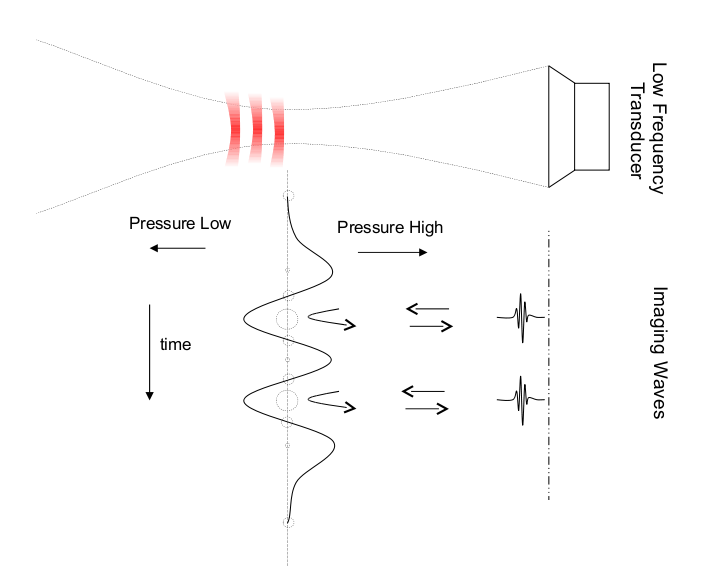
\includegraphics[width=0.8\textwidth]{change_radius.png}}
%      \hspace{1cm}
%      \subfloat[By timing a high frequency wave to meet the bubble
%      while it is under the influence of the low-frequency wave, the
%      bubble can be induced to resonate at higher than usual
%      frequencies. This is because the bubble will transiently be
%      smaller (when it is compressed) and because it will experience a
%      Doppler shifted imaging wave. ]{
%           \label{fig:both_waves}
%           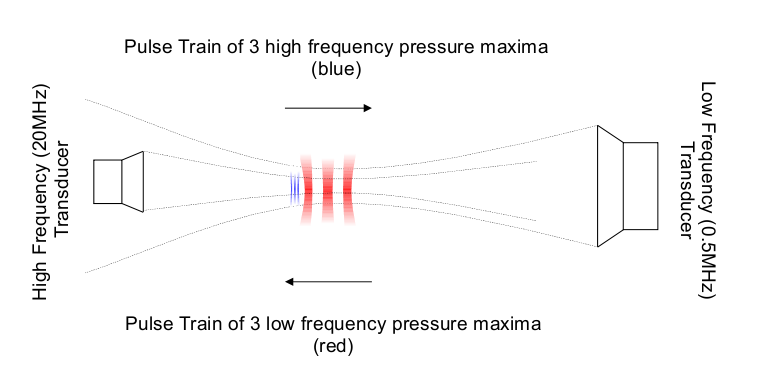
\includegraphics[width=0.8\textwidth]{both_waves.png}}
%      \caption{Low and high frequency pulses emitted.
%      }
%      \label{fig:general_idea}
% \end{figure}

% \begin{figure}[h]
%      \centering
%           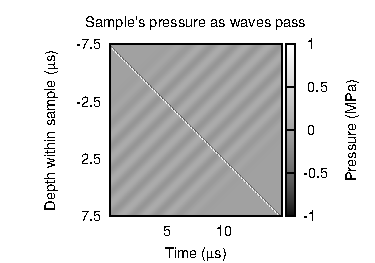
\includegraphics[width=0.8\textwidth]{pulses.pdf}
%      \caption{
%        The incident pressure wave resulting from the superposition of
%        the low frequency and imaging waves as a function of sample
%        depth.
%        Negative depths are closer to the imaging transducer.
%      }
%      \label{fig:pulses}
% \end{figure}

% \begin{figure}[h]
%      \centering
%           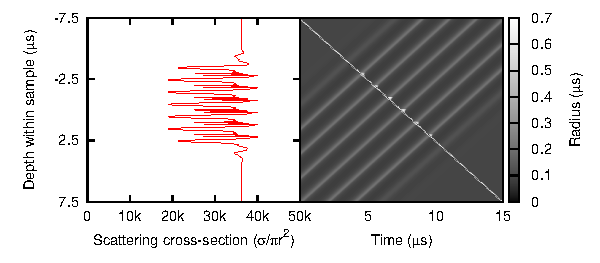
\includegraphics[width=1.0\textwidth]{radxs.pdf}
%      \caption{Normalised scattering cross section of a bubble as a
%        function of depth,
%        plotting with the corresponding radial response for the pulses
%        as drawn in \figref{pulses}.
%      }
%      \label{fig:xs}
% \end{figure}


%\begin{figure}[h]
%     \centering
%     \subfloat[]{
%     \missingfigure{The sketch of the arrangement}\label{fig:pressure_pulses:a}
%   }\\
%     \subfloat[]{
%     \missingfigure{The incident pressures}\label{fig:pressure_pulses:b}
%}\\
%     \subfloat[]{
%     \missingfigure{The generated response}\label{fig:pressure_pulses:c}
%   }
%     \caption{
%       When the transducers face each the phase relationship between the two pulses will be sampled as a function of depth.
%       \subref{fig:pressure_pulses:a} shows the arrangement of the transducers.
%       \subref{fig:pressure_pulses:b} shows the pulses pass through each other as a function of depth and time.
%       The acoustic response of a bubble at each depth is illustrated in \subref{fig:pressure_pulses:c}.
%     }
%     \label{fig:pressure_pulses}
%\end{figure}

In this thesis two separate ultrasound transducers are used to generate the cavitating and imaging waves.
This brings the advantage of flexibility:
the characteristics of the cavitating and imaging waves are completely decoupled.
The  frequency, pulse-duration, focal depth and duty-cycle of each pulse can be chosen and interchanged independently,
and without  compromise with regard to a crystal's bandwidth or curvature.
%that  arises when generating the pulses from a single crystal or a set of interleaved crystals.
%Additionally, by separating the driving and imaging waves
%the properties of the driving or imaging wave can be easily switched.

To investigate the phase-relationship between the driving and imaging pulses
when incident upon a bubble,
the two waves must pass simultaneously through a bubbly fluid situated at the common focus.
This is most easily achieved by  having the two transducer's facing
each other. %, as illustrated by the cartoon of \figref{general_idea}.
If the bubbly mixture is both dense and homogeneous,
so that it may be considered a continuous medium,
then at every position within the sample a different phase relationship
between the two waves is interrogated.
\todo{Maybe dig out the picture here}
Temporal alignment was achieved as follows.
The two transducers were fired from the same trigger pulse and the time lag between the two pulse arrival times was found.
The lag is due to the imaging transducer having a shorter focal length,
and gives the time for which the imaging transducer needs to be delayed.
This delay was achieved with  a second pulse generator, as shown in \figref{arrB}.
The phase relationship at different distances between the two transducers was then found by moving the hydrophone
 along the (approximate) co-axis of the two transducers.
The voltage-time waveforms from tracking the hydrophone across the focus are shown in \figref{phases}.
\Figref{phase_exp_a} should help with the interpretation of \figref{phase_exp_b} 
by showing only a few of the hydrophone traces recorded.
Each subsequent trace from left to right gives the pressure recorded by the hydrophone for a particular distance along the co-axis.
Quick time is the time coordinate measured in each such trace,
while the distance along the co-axis is measured in microseconds away from the co-focus, which is set as the origin.
The traces more to the left are when the hydrophone is on the imaging transducer's side of the focus.
We in fact took 600 traces over 6\milli\metre\ and it becomes simpler to view the graph from above in a grey-scale for acoustic pressure.
This is done in \figref{phase_exp_b}.  
%Again, the traces to the left are recorded on the imaging transducer's side of the focus.
%The origin, in both plots is taken to be the co-focus.
%Notice that in \figref{phases} the  6\milli\metre\ over which the measurements took place have been rewritten in terms of the time of flight.
The rewriting of all distances in terms of time of flight is convenient as the plots then become 
independent of the (temperature dependent) speed of sound.
%Sound then travels across the plot at 45\degree,
%and the two incident waves meet on the plot at 90\degree.
%Using the fact that the two incident sound fields are orthogonal to each other (in the sense of the plot),
%makes it easier to see that phase is maintained throughout the sample,
%and will not be averaged out by a large number of scatterers\footnote{\label{important_footnote}
%That the phase information will not be averaged out over the large number of bubbles in a sample
%assumes that we have a constant speed of sound in the sample.
%For a bubbly liquid this is not true, as
%fluctuations in bubble density will cause the speed of sound to vary.
%A twenty megahertz wave, with a wavelength of about 75\micro\metre, may be averaged away
%over a distance of, say,  10\micro\second\ if there is a change in the speed of sound of about
%\eq{
%  \Delta c = \frac{35\micro\metre}{10\micro\second} = 3.5\metre\second^{-1}.
%}
%This is feasible, and we therefore need to be careful not to let our densities get too large.
%}.


\begin{figure}[p]%[htp]
  \centering

  \subfloat[Hydrophone measurements of the pressure-time waveforms at various distances along the acoustic axis within the co-focal region.]{
    \label{fig:phase_exp_a}
    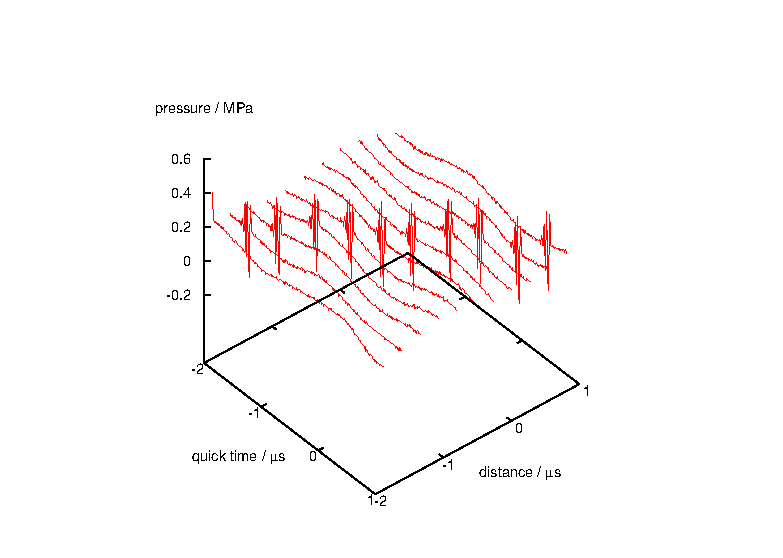
\includegraphics[width=.8\textwidth]{15_exp.eps}
    }\\
  \vspace{.3in}
  \subfloat[Gray scale representation showing many more sampling points.]{
    \label{fig:phase_exp_b}
    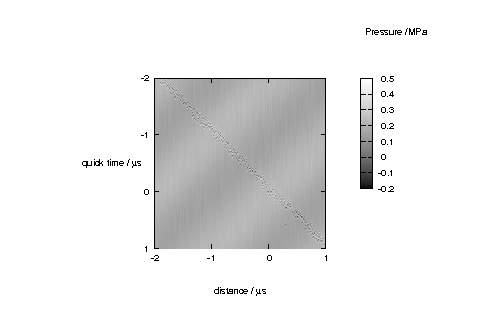
\includegraphics[width=1.0\textwidth]{exp_theory.eps} %[width=.8\textwidth ]
    }
  \caption{     %A sanity check.  
    %A comparison between a simple model of the phase relationship and the corresponding experimentally obtained values.
    The phase relationship between the waves from the two transducers.
    The imaging transducer is to the left, facing the pumping transducer (as in \figref{arrangements}).
    Each line \figref{phase_exp_a} represents a recording on a hydrophone placed in between the two transducers.
    The `distance' is measured in microseconds so that the graph is independent of the speed of sound (which can be considered to be set to unity).
    Both axes are measured with respect to an origin placed at the co-focus.}
  \label{fig:phases}
\end{figure}


Finally the hydrophone needs to be accurately replaced with the sample holder.
This was done by finding the transit time for a high frequency pulse to echo off the hydrophone.
%The hydrophone here can be considered as negligibly thin.
When the hydrophone is replaced with the sample holder, another pulse echo time is recorded.
The position of the sample is then adjusted so that the co-focus found with the hydrophone lies at the centre of the  sample holder.
 



%This is illustrated in \figref{pressure_pulses:a}.
%Bubbles that are close to the imaging transducer will backscatter sound
%before the driving wave arrives.  This is seen in the top left of \figref{pressure_pulses:b}.
%The forward scatter contributed by these bubbles from the driving wave arrives later, as seen in the top right of \figref{pressure_pulses:b}.
%Bubbles that are a little further away will be driven by the driving  and  imaging waves simultaneously.
%Still further from the imaging wave, the driving wave will arrive first, followed by the imaging wave.
%%Further from the away still, theThe first few oscillations will be due to the driving wave alone,
%%before the  imaging wave arrives at a given phase of the driving wave.

Alternative arrangements for the two transducers are possible.
In principle, the two transducers could be at any angle, $\phi$, with respect to each other.
However, having the transducers co-axial (where $\phi = 0\degree,180\degree$) is optimal because
the sampling precision in the axial direction is vastly superior than in the orthogonal directions.
This is because the sampling rate in the axial direction is determined by the rate at which samples can be digitalised.
In the orthogonal direction sampling precision  is determined by the beam width of the ultrasound transducer.
Any arrangement other than co-axial will therefore deteriorate the sampling precision by a factor of $\sin(\phi)$.

The two co-axial arrangements both have their advantages and dissadvantages.
The advantage of having the two transducers facing each other ($\phi = 180\degree$) 
is that all phase relationships between the two pulses are explored in a single shot.
The disadvantage is that the driving pulse is incident upon the imaging transducer even if no scattering occurs.
This directly transmitted signal is not generally dominant, however, so long as the  band-widths of the driving and imaging crystals do not greatly overlap.

If the two crystals are interleaved into the same transducer ($\phi = 0\degree$) then the two pulses traverse with each other.  
There is no problem with either signal being directly transmitted.
However, each phase relation of the two pulses needs to be carried out individually
and it is difficult to maintain a population of micron-sized bubbles in a consistent state for any length of time.
A further problem is that the phase relationship between the two pulses changes as a function of density;
a high frequency pulse {\em surfing} on a compression of a lower-frequency pulse travels at a greater speed than when timed with a rarefaction.
This effect is measurable and is the basis of {\surf}-imaging\cite{Anderson}\todo{get citations}.
Finally, interleaving two crystals into the same transducer generally requires bespoke transducers
and comes at a considerable cost.
For these reasons, the angle $\phi = 180\degree$ is chosen in this thesis.


\section{The source of bubbles}\label{sec:WE:why_water}

\begin{figure}[t]%
  \centering
    % GNUPLOT: LaTeX picture with Postscript
\begingroup
  \makeatletter
  \providecommand\color[2][]{%
    \GenericError{(gnuplot) \space\space\space\@spaces}{%
      Package color not loaded in conjunction with
      terminal option `colourtext'%
    }{See the gnuplot documentation for explanation.%
    }{Either use 'blacktext' in gnuplot or load the package
      color.sty in LaTeX.}%
    \renewcommand\color[2][]{}%
  }%
  \providecommand\includegraphics[2][]{%
    \GenericError{(gnuplot) \space\space\space\@spaces}{%
      Package graphicx or graphics not loaded%
    }{See the gnuplot documentation for explanation.%
    }{The gnuplot epslatex terminal needs graphicx.sty or graphics.sty.}%
    \renewcommand\includegraphics[2][]{}%
  }%
  \providecommand\rotatebox[2]{#2}%
  \@ifundefined{ifGPcolor}{%
    \newif\ifGPcolor
    \GPcolortrue
  }{}%
  \@ifundefined{ifGPblacktext}{%
    \newif\ifGPblacktext
    \GPblacktexttrue
  }{}%
  % define a \g@addto@macro without @ in the name:
  \let\gplgaddtomacro\g@addto@macro
  % define empty templates for all commands taking text:
  \gdef\gplbacktext{}%
  \gdef\gplfronttext{}%
  \makeatother
  \ifGPblacktext
    % no textcolor at all
    \def\colorrgb#1{}%
    \def\colorgray#1{}%
  \else
    % gray or color?
    \ifGPcolor
      \def\colorrgb#1{\color[rgb]{#1}}%
      \def\colorgray#1{\color[gray]{#1}}%
      \expandafter\def\csname LTw\endcsname{\color{white}}%
      \expandafter\def\csname LTb\endcsname{\color{black}}%
      \expandafter\def\csname LTa\endcsname{\color{black}}%
      \expandafter\def\csname LT0\endcsname{\color[rgb]{1,0,0}}%
      \expandafter\def\csname LT1\endcsname{\color[rgb]{0,1,0}}%
      \expandafter\def\csname LT2\endcsname{\color[rgb]{0,0,1}}%
      \expandafter\def\csname LT3\endcsname{\color[rgb]{1,0,1}}%
      \expandafter\def\csname LT4\endcsname{\color[rgb]{0,1,1}}%
      \expandafter\def\csname LT5\endcsname{\color[rgb]{1,1,0}}%
      \expandafter\def\csname LT6\endcsname{\color[rgb]{0,0,0}}%
      \expandafter\def\csname LT7\endcsname{\color[rgb]{1,0.3,0}}%
      \expandafter\def\csname LT8\endcsname{\color[rgb]{0.5,0.5,0.5}}%
    \else
      % gray
      \def\colorrgb#1{\color{black}}%
      \def\colorgray#1{\color[gray]{#1}}%
      \expandafter\def\csname LTw\endcsname{\color{white}}%
      \expandafter\def\csname LTb\endcsname{\color{black}}%
      \expandafter\def\csname LTa\endcsname{\color{black}}%
      \expandafter\def\csname LT0\endcsname{\color{black}}%
      \expandafter\def\csname LT1\endcsname{\color{black}}%
      \expandafter\def\csname LT2\endcsname{\color{black}}%
      \expandafter\def\csname LT3\endcsname{\color{black}}%
      \expandafter\def\csname LT4\endcsname{\color{black}}%
      \expandafter\def\csname LT5\endcsname{\color{black}}%
      \expandafter\def\csname LT6\endcsname{\color{black}}%
      \expandafter\def\csname LT7\endcsname{\color{black}}%
      \expandafter\def\csname LT8\endcsname{\color{black}}%
    \fi
  \fi
  \setlength{\unitlength}{0.0500bp}%
  \begin{picture}(5760.00,3528.00)%
    \gplgaddtomacro\gplbacktext{%
      \csname LTb\endcsname%
      \put(1210,704){\makebox(0,0)[r]{\strut{} 0}}%
      \put(1210,1002){\makebox(0,0)[r]{\strut{} 0.05}}%
      \put(1210,1300){\makebox(0,0)[r]{\strut{} 0.1}}%
      \put(1210,1598){\makebox(0,0)[r]{\strut{} 0.15}}%
      \put(1210,1896){\makebox(0,0)[r]{\strut{} 0.2}}%
      \put(1210,2193){\makebox(0,0)[r]{\strut{} 0.25}}%
      \put(1210,2491){\makebox(0,0)[r]{\strut{} 0.3}}%
      \put(1210,2789){\makebox(0,0)[r]{\strut{} 0.35}}%
      \put(1210,3087){\makebox(0,0)[r]{\strut{} 0.4}}%
      \put(1342,484){\makebox(0,0){\strut{} 0}}%
      \put(1887,484){\makebox(0,0){\strut{} 2}}%
      \put(2432,484){\makebox(0,0){\strut{} 4}}%
      \put(2977,484){\makebox(0,0){\strut{} 6}}%
      \put(3522,484){\makebox(0,0){\strut{} 8}}%
      \put(4067,484){\makebox(0,0){\strut{} 10}}%
      \put(4612,484){\makebox(0,0){\strut{} 12}}%
      \put(5157,484){\makebox(0,0){\strut{} 14}}%
      \put(308,1895){\rotatebox{-270}{\makebox(0,0){\strut{}number density (normalised)}}}%
      \put(3385,154){\makebox(0,0){\strut{}bubble radius (microns)}}%
    }%
    \gplgaddtomacro\gplfronttext{%
      \csname LTb\endcsname%
      \put(4442,2914){\makebox(0,0)[r]{\strut{}15:08}}%
      \csname LTb\endcsname%
      \put(4442,2694){\makebox(0,0)[r]{\strut{}17:39}}%
      \csname LTb\endcsname%
      \put(4442,2474){\makebox(0,0)[r]{\strut{}20:10}}%
      \csname LTb\endcsname%
      \put(4442,2254){\makebox(0,0)[r]{\strut{}22:41}}%
      \csname LTb\endcsname%
      \put(4442,2034){\makebox(0,0)[r]{\strut{}25:12}}%
      \csname LTb\endcsname%
      \put(4442,1814){\makebox(0,0)[r]{\strut{}27:44}}%
    }%
    \gplbacktext
    \put(0,0){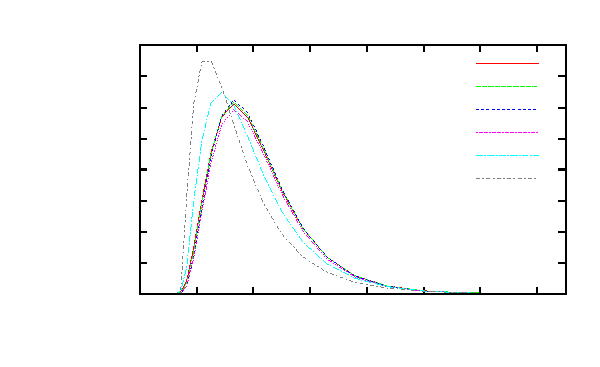
\includegraphics{sonovue_sizes}}%
    \gplfronttext
  \end{picture}%
\endgroup

  \caption{
    \Sonovue\ distribution at various times after manufacture (in minutes).
  }
  \label{fig:sonovue_sizes}
\end{figure}


There are a number of microbubble sources that could be used to test the influence of the low frequency wave 
on the imaging wave.

%\subsection{A bubble generated from a perflurocarbon emulsion}


%Each of these methods have their respective advantages.
\desc{
\item[A bubble generated from a perflurocarbon emulsion:]\hfill \\
  It seems likely that perfluorocarbon droplets will 
  eventually be able to leave the blood and be vapourised in situ to generate a contrast agent (see \chapref{introduction}).
  Testing two wave imaging using a bubble perfluorcarbon emulsion would
  therefore represent a natural end to this research project:
  the technique tested in the domain in which it is most useful,
  a cavitating wave acting upon a sub-micron bubble.
  Perfluorocarbon emulsions do not, however, represent a natural beginning.

  The technology in developing such contrast agents is still young.
  Most of the success so far has been with larger droplet sizes (greater than \unit{400}\nano\metre\todo{cite})
  while manufacturing smaller droplet sizes, required for producing an extravacularised bubble of less than \unit{400}\nano\metre\todo{radius or diameter},
  has remained troublesome\todo{cite} (although see \todo{cite}).
  The pressures that have hitherto been used to generate the bubbles are above ...\todo{get this number}, far in excess of those used in diagnostic applications,
  with cavitating pulse lengths of ...\todo{get number} cycle.
  Such pressures require the emulsion to be prepared in exceptionally clean water
  to be sure that the bubbles generated by the driving wave are not simply from heterogeneous nucleation of the water.
  Furthermore, any surfactant used to stabilise the emulsion must be known not to also stabilise
  any bubble formed in the manufacturing process, or to itself form a nucleating centre.
  Research is being carried out by other groups \todo{cite} to reduce the pressure required for to cavitate a perlfuorocarbon droplet by mixing different perfluorocarbons,
%  which ideally would be possible with a diagnostic transducer,
  but this research has not yet come to fruition \todo{cite}.
  


%\subsection{Commercially available microbubbles}
\item[Commercially available microbubbles:]\hfill \\
  The difficulties resulting from the novelty of perfluorocarbon  emulsions 
  are not present for commercial available microbubbles.
  Microbubble contrast agents have been licensed since ,\todo{get date and bubble}
  and \Sonovue\ (Bracco) is currently licenced for clinical use in the EU \todo{cite}.
  Both its size distribution (...\todo{get numbers and cite}) 
  and its resonances \todo{cite}  are well characterised.

  However, the size distribution of commercial microbubbles causes problems in this experiment.
  Firstly, the mean radius of the bubbles is greater than a micron.
  This means that the bubbles float, albeit slowly, making a distribution of bubbles
  that is homogeneous both spatially and temporally difficult to achieve.
  Even if the bubbles are circulated, the larger bubbles are gradually lost in the experiment.
  The results of a preliminary experiment showing the size distribution of \Sonovue\ circulating 
   through a Mastersizer is shown in \figref{sonovue_sizes},
  and other studies show similar results\todo{cite}.
  Since microbubbles are highly attenuating to ultrasound \todo{cite}
  the pressure field in the sample changes as the distribution changes,
  meaning that the response becomes a complicated function of depth.
  %The large size of commercial bubbles also means that they are more fragile to larger pressures.
  %\todo[inline]{Comment about curvature to back this up}
  %


  Secondly, commercial microbubbles have a fairly broad distribution of sizes.
  This causes problems because the phase offset between the bubble's pulsations and  cavitating wave 
  is a function of the bubble's size (see \chapref{computations}).
  The scale of this problem can be understood from \figref{phase_radial} on page \pageref{fig:phase_radial}.
  Not only would we be trying to find the excess scattering cross-section of  a bubble in the complicated region
  corresponding to large bubble radii, we would be trying to perform a weighted average over that region.

Finally, the use of microbubbles forces the experiment away from the domain where a submicron bubbles is generated  with a high pressure wave.
  
  %Finally, the degree to which the samples are free from nucleation centres is uncertain with commercial bubbles.
  %The bubbles are designed to be sterile, and come packaged with a dry surfactant and a solution into which the bubbles are to be formed.
  %Making a control solution to test that you are actually imaging the commercial bubble and , free from the comertial 
  %Most bubbles are formed from by injecting 
  %so need to use a control.
  %setting up a control is difficult.
  %This is particulaly the case for contrast agents such as levovist 
  %that often has undisovled honeycomb left in the sample.
  %Distinguishing between microbubble bubble and heterogenous nucleation difficult.


%\subsection{Heterogeneous nucleation of tap water}


\item[Heterogeneous nucleation of tap water:]\hfill \\
  The heterogeneous nucleation of tap water is perhaps the simplest method of generating a bubble.
  Indeed, it makes a good control method to the more elaborate techniques above.
  It is also the method that most closely matches the ideal parameters for cavitating an extravascular contrast agent.
  With relatively short pulses (less than 10 cycles) at pressures that are achievable with diagnostic ultrasound transducers 
  (less than approximately \unit{1}\mega\pascal\ peak-negative pressure)
  gas entrapped in stabilised microbubbles and motes can be released\todo{cite}.
  %(An example is shown if \figref{av:108:1000_ex} and is discussed in \secref{WE:motivating_ex}).
  
  The critical radius, $R$, as a function of acoustic pressure, $P$, for an air bubble in water was estimated in \chapref{nucleation}.
  %of a bubble generated by  can be estimated from the Laplace pressure
  %\eq
  %{
  %  R = \frac{2\sigma}{P}
  %}
  %where $\sigma$ is the surface tension between air and water,
  %and $P$ is the applied pressure. 
  If the negative pressure is  $\unit{1}\mega\pascal$ then the diameter of the bubble is approximately $300\nano\metre$
(\figref{} on page \pageref{}).
  This is the size that would be expected for extravascular contrast agent,
  achieved with a pressure that would be desirable for an extravascular contrast agent.
  %It therefore makes an excellent mode
  %Should such bubbles exist in the tap water,
  %then submicron bubbles can be elicited at diagnostic pressures.
  Furthermore, tap water is homogeneous and is stable indefinitely once it has reached a stable equilibrium,
  at least up until the sample has been pulsed with an ultrasound wave.
  
  %It is for this reason that tap water is troublesome when cavitation within the sample is not desired - neither.
  Tap water provides a very good source of bubbles for testing the use of a cavitating wave in controlling the scattering of an imaging wave.
}  
This chapter uses tap water as a source of bubbles.
The bubbles in the medium are therefore generated by heterogeneous nucleation of the water.
At diagnostic ultrasound pressures, 
this implies type III and type IV nucleation (see  \chapref{nucleation}).
%Motivation for using bubbles obtained from tap water
%rather than from other sources
%is given in \secref{WE:why_water}.
The characterisation of the water medium adds 
requirements to the experimental method
that are additional to those needed to test the influence of the cavitating wave on scattering of the imaging wave.
A full list of the experimental objectives is given in  \secref{WE:objectives}
and the experimental methodology designed to meet these objectives is given in \secref{WE:methodology}.




\section{Experimental Objectives} \label{sec:WE:objectives}

This thesis has five experimental objectives that aim to test the predictions made in the first parts of the thesis.
\nlist{
\item Determine whether bubbles can be evacuated from dirty water with a driving wave,
  and subsiquently detected with a higher-frequency pulse.
\item Determine whether an evacuated bubbles can be {\em imaged by pulse echo} 
  with a  higher-frequency pulse.
\item Determine if the precise location of the bubble can be determined.
  In particular, can the excess scatter introduced in \chapref{computations}
  be shown to have experimental merit?
\item Determine whether any of the characteristics of the bubble can be inferred from the scattered sound.
  In particular, can the pressure of the driving wave be used to determine the radius of the bubble
  as hoped in \chapref{nucleation}?
  Can  the lifetime of the bubble be measured by using the driving-imaging wave pair, which would in turn give a second estimate of the radius?
\item 
  Determine whether the acoustic Keller-Miksis equation derived in \chapref{measurement} improves the modelling of the returned echo.
}

The objectives are incremental in that the latter depend upon the former.
The first is the most straightforward.
The generation of bubbles in dirty water is familiar to most practicioners of ultrasound
and the only technical difficulty is in timing the imaging wave appropriately to image the wave.

The second question is much more difficult.
For the second question we wish to show that the evacuated bubble interacts acoustically with the imaging wave.
Sound that is radiated when the bubble is generated is no longer of interest.
The third asks whehter the excess pressure technique of \chapref{computations} is a viable means of locating a bubble, 
and thereby conclusively demonstrating the acoustic interaction of nucleated bubble with the imaging wave.

The final two questions are the most challenging of all because they require
the measurement of bubble specific parameters from within larger population.
Such questions will only be answerable if the large  spread found in parameters such
as the radius (\figref{}) is not representative of the spread found in the bubbles that interact acoustically.
Since in this thesis the focus is on diagnostic pulses, 
which are typically limited to being a few cycles long,
questions three and four are not expected to yield good results.
The range of frequencies contained in the pulses are too great to hope for narrow resonance characteristics in the population of generated bubbles.

\section{Experimental Protocol}\label{sec:exp:protocol}

The broad design of the experiments to test these objectives are now presented.

In \secref{exp:prelim}, a preliminary study is discussed that 
confirms question 1 in the affirmative.
It is found, however, that the preliminary study is not capable of determining the answer to 
the second question, namely,
whether the imaging transducer actively imaging the generating bubbles
or whether it is simply passively detecting high harmonics
of bubbles oscillating due the driving wave.
This prompts some changes in experimental design that are discussed in \secref{exp:finalDesign}.
%that bubbles could be freed from the motes within tap water and detected with a higher frequency wave.


\subsection{Preliminary study: The generation and detection of bubbles in dirty water}\label{sec:exp:prelim}

The primary goal of the preliminary study was  to determine whether bubbles could be evacuated from motes in tap 
water with a low frequency wave, 
and whether evidence for this could be detected with a high frequency wave.

For this purpose a \unit{0.5}\mega\hertz\ transducer (TMS, focal length: \unit{50}\milli\metre) was chosen to evacuate the gas from the water,
and a \unit{20}\mega\hertz\ (Panametrics, focal length: \unit{50}\milli\metre \todo{Obtain focal length})  transducer was used for imaging.
These transducers were chosen for a number of reasons:
\nlist{
  \item It was hoped that the frequency ratio of 40 between these transducers 
    would help eliminate direct transmission from the driving wave to the imaging transducer.
  \item  \unit{0.5}\mega\hertz\ was chosen  for the driving wave because it is below the principle resonances of the bubbles that are expected to be evacuated in the fluid (\figref{}).
The motivation for being below the principle resonance comes from \chapref{computations} where it was found that the interactions between the driving and imaging  waves become hard to interpret at resonance.
\item  \unit{20}\mega\hertz\ was chosen for the imaging wave because  \unit{20}\mega\hertz\ should  resonate free gas bubbles of about \unit{300}\nano\metre (\figref{}).
This is approximately the size of bubble  that we ultimately wish to image.
\item Both transducers are  focussed.  Firstly, this results in an imaging volume that is well located.
Secondly, higher driving and imaging pressures can be obtained at the focus than would be possible if the transducers were flat.
A plot of the focal widths is provided in \figref{}.  
\item The \unit{20}\mega\hertz\ trasnducer was a spare taken from a  Cortex Skin Scanner
that had been customised to obtain the radio-frequency output.
  The transducer could therefore be fixed to obtain M-mode images,
  or mounted on a pendulum  scan-head to obtain B-mode images.
 }

The two transducers were clamped together in a custom made sample holder which ensured that the mechanical focus of the two transducers was conincident.  
Two mounts for the imaging transducer were made, one that fixed the imaging transducer on axis with the driving transducer, and one that enabled the imaging trasducer to swing for B-Mode imaging.
The cofocus was designed so that it stood in the middle of a sampling volume that could be separated from the transducer standoffs with Mylar film.  
\Figref{} gives a schematic of the holder.


B-mode imaging was chosen for the preliminary study
so as to  maximise the view of the two wave interaction.
%In order to maximise the chance of imaging any bubbles within the medium 
%the imaging transducer was used in 2-dimensional mode.
%This helped to mitigate the risk of missing regions of the cavitation chamber that were generating bubbles. 
The modified  Cortex scanner gives output to the frame trigger output, the
A-line trigger output , the
direction of the scan of the transducer and the RF data.
It has a slow frame rate of  approximately \unit{3-4}\hertz.
The cortex also has a curious although very useful pulse sequence, with two
A-line-pulses in rapid (100 microsecond) succession, followed by a large (millisecond
scale) interval.
This is illustrated in \figref{cortex_gate}.

\begin{figure}[h]
     \centering
          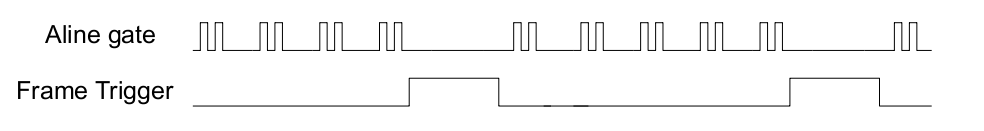
\includegraphics[width=0.8\textwidth]{cortex_gate.png}
     \caption{The cortex fires two A-lines in quick succession before
       repeating the sequence after a
     relatively large pause.}
          \label{fig:cortex_gate}
\end{figure}


The focal length of the low frequency transducer is longer than that
of the Cortex
transducer
and as such it needs to be triggered before the cortex in order for
both signals to reach the sample at the same time.
It is therefore impossible to time the low frequency transducer to
propagate through to the sample  at the same time as the low
frequency pulse.
The two pulses from the cortex enables this problem to be overcome.
The first pulse of the cortex A-line doublet is used to trigger 
a timer delay for the low frequency transducer.
The delay is chosen  so that the first low frequency pulse arrives at the
sample at the same time as the second high frequency pulse.
In this way one  generates two interleaved images, with adjacent A-lines
imaged with the pulse off, and then the pulse on.
The second low frequency pulse  (triggered from the second
A-line doublet) is ignored.
The electronic arrangement of the preliminary experiment is summarised in \figref{}.




% Sound can return from a scatterer via a number of different mechanisms.
% First it can be back-scattered, where reflections are generated by changes in acoustic impedance, 
% typically where there is a change in density of the medium.
% Secondly, new sources of sound  can also be induced by the incident pressure wave.
% These new sources can be the translational oscillations forced upon an object, 
% where a difference in density causes it to bob back and forth in the sound field.
% Additionally, oscillatory changes in volume and shape can be induced, generating a secondary acoustic field.
% These  oscillations in volume typically result from a difference  in compressibility with respect to the external medium.
% It is this final mechanism that usuaslly dominates.


% There is a very strong frequency dependence to the oscillation of compressible scatterers,
% and this is conveniently expressed as the ratio of scattering to geometric cross-section (i.e. $\sigma/\pi a^2$, where $a$ is the bubble radius.).
% Inasmuch as the incident pressure wave is low in amplitude, 
% so that sound propagation is linear and scatterer oscillation remains radial,
% the scattering cross-section can be expressed as a series expansion of spherical harmonics,
% constrained so that  both the pressure and the radial velocity are continuous on the bubble wall.
% In the simplest case the effects of surface tension and viscosity are ignored.
%was considered by \cite{Anderson1950}\footnote{See \cite{Feuillade1999} for a modern discussion of Anderson's results}.
% The relative cross-section for a free air bubble and for a perfluoropentane liquid drop under this model 
% \citep{Anderson1950}\footnote{See \cite{Feuillade1999} for a modern discussion of Anderson's results} are plotted in \figref{cross_sections},
% where the expansion has been carried out to $10^{\mbox{th}}$ order.
% %\begin{center}
% \begin{figure}[h]%[htp]
%   \centering
%   \subfloat[Scattering cross section for an air bubble]{
%     \label{fig:CSbubble}
%     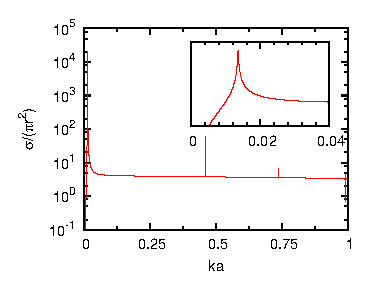
\includegraphics[width=.4\textwidth]{bubble.eps}}
%    \hspace{.3in}
%    \subfloat[Scattering cross section for a perfluoropentane liquid drop ]{
%     \label{fig:CSpfp}
%     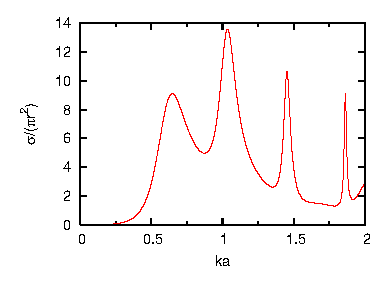
\includegraphics[width=.4\textwidth]{pfp.eps}}
%   %\hspace{.3in}
%    \caption{
%      Scattering cross sections resulting from a tenth order series solution of \cite{Anderson1950}.
%    }
%    \label{fig:cross_sections}
% \end{figure}
% %\end{center}

% Notice first that the scattering for the gas bubble is orders of magnitude larger than for for liquid drop.
% This is due to much larger difference in compressibility between liquid-gas than between liquid-liquid,
% and it is this that makes gas bubbles useful as ultrasonic contrast agents.
% A second point of interest is that, due to the low density of gas compared to the medium,
% the first resonance peak of the (Mie) analysis of \figref{CSbubble}
% has shifted to the small value of  $ka=0.013$ where $k$ is the wavenumber and $a$ is the bubble radius.
% %This is because the difference in compressibility between a liquid and gas can be up to seven orders of magnitude,
% %whereas a three order of magnitude difference in density is typical.
% %Oscillatory expansions and contractions, then, dominate scattering for gas bubbles,
% %and in the main this is what is meant when we talk of reflected or scattered sound.
% %Mostly this abuse of language is convenient and causes few problems.
% %Notice that the low density of air bubbles with respect to the water medium shifts the first resonsnace peak of this (Mie)
% %analysis down to a value of $ka=0.0134$ where $k$ is the wavenumber.

% The model of \cite{Anderson1950}, then, results in a resonance frequency, $f_0$, that is inversely proportional to the bubble radius,
% \eqal{
%   f_0 &= \frac{\omega}{2\pi} = \frac{0.0134 c}{2\pi} \frac{1}{a} \nonumber\\
%       &\approx \frac{3.2}{a}\metre\second^{-1},
% }{graph_res}
% where a speed of sound of  $1500\metre\second^{-1}$ has been used.
% This relation was derived by \cite{Minnaert1933}, who found
% \eql{
%   f_0 = \frac{1}{2\pi r}\sqrt{\frac{3\gamma p}{\rho}},
% }{Minnaert}
% where $p$ is the pressure within the bubble, $\rho$ is the density of the medium,
% and $\gamma$ is the adiabatic index.
% That \eqnref{Minnaert} does in fact reduce to \eqnref{graph_res} in standard conditions can be confirmed
% by substituting in the atmospheric pressure, $p=101\kilo\pascal$, the density of water, $\rho = 998\kilo\gram\per\metre\cubed$ and 
% the adiabatic constant for an ideal diatomic gas, $\gamma = 1.4$.







%I have done cavitation experiments for lots of different driving pressures.
%These pressures are recorded in my notes in terms of the number of decibels that the electric signal to the amplifier was suppressed.
%Since the number of pressures tried was great, and since beam plots takes a long time,
%I have only done axial  beamplots for 4 of the pressures tried.

%\Figref{water_cavitation_70} indicates the cavitation events recorded at 30db suppression.
%I have the (geometric) axial beam plot for this pressure.
%I have the code to process the beamplot data (to indicate the pressure at each location in th image, 
%although this code is untested and I haven't done the final step to actually draw it on the data.
%This final step - all being well- shouldn't take long. 
%It is my task, I think, for as soon as this document is finished.


\subsubsection{Results of the preliminary study}

Pressures chosen \todo{Not sure what to do here}

%This helped This helped to reduce the chances of 





\begin{figure}[h]
     \centering
          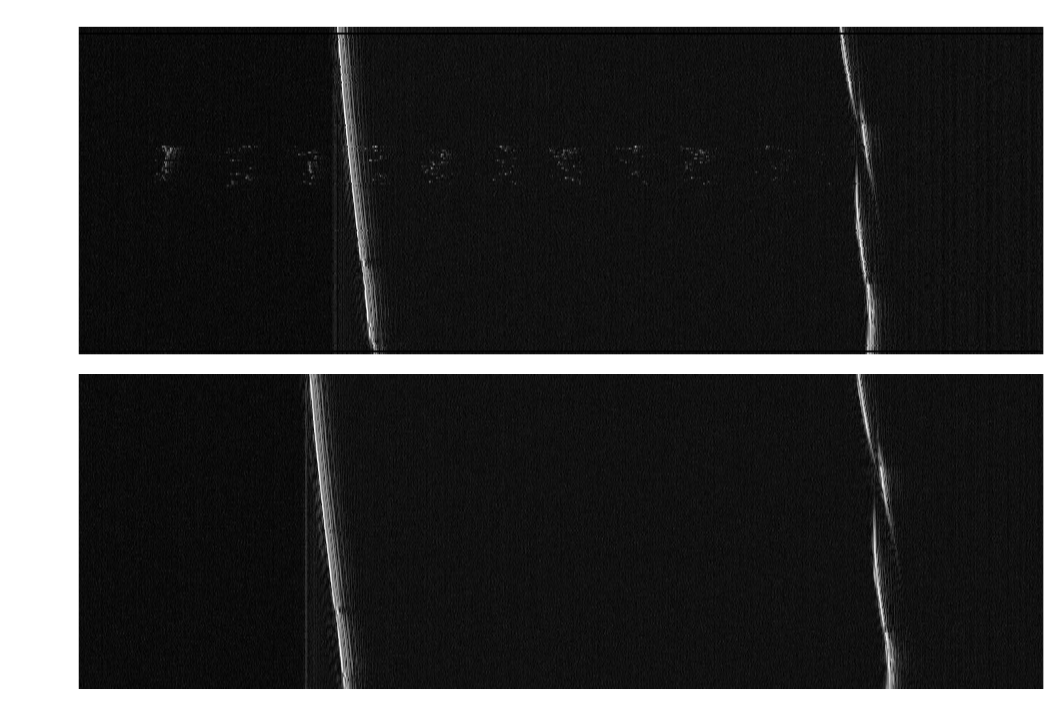
\includegraphics[width=0.8\textwidth]{rotterdam_02_water.png}
     \caption{30db}
   \label{fig:water_cavitation_70}
\end{figure}


\begin{figure}[h]
     \centering
          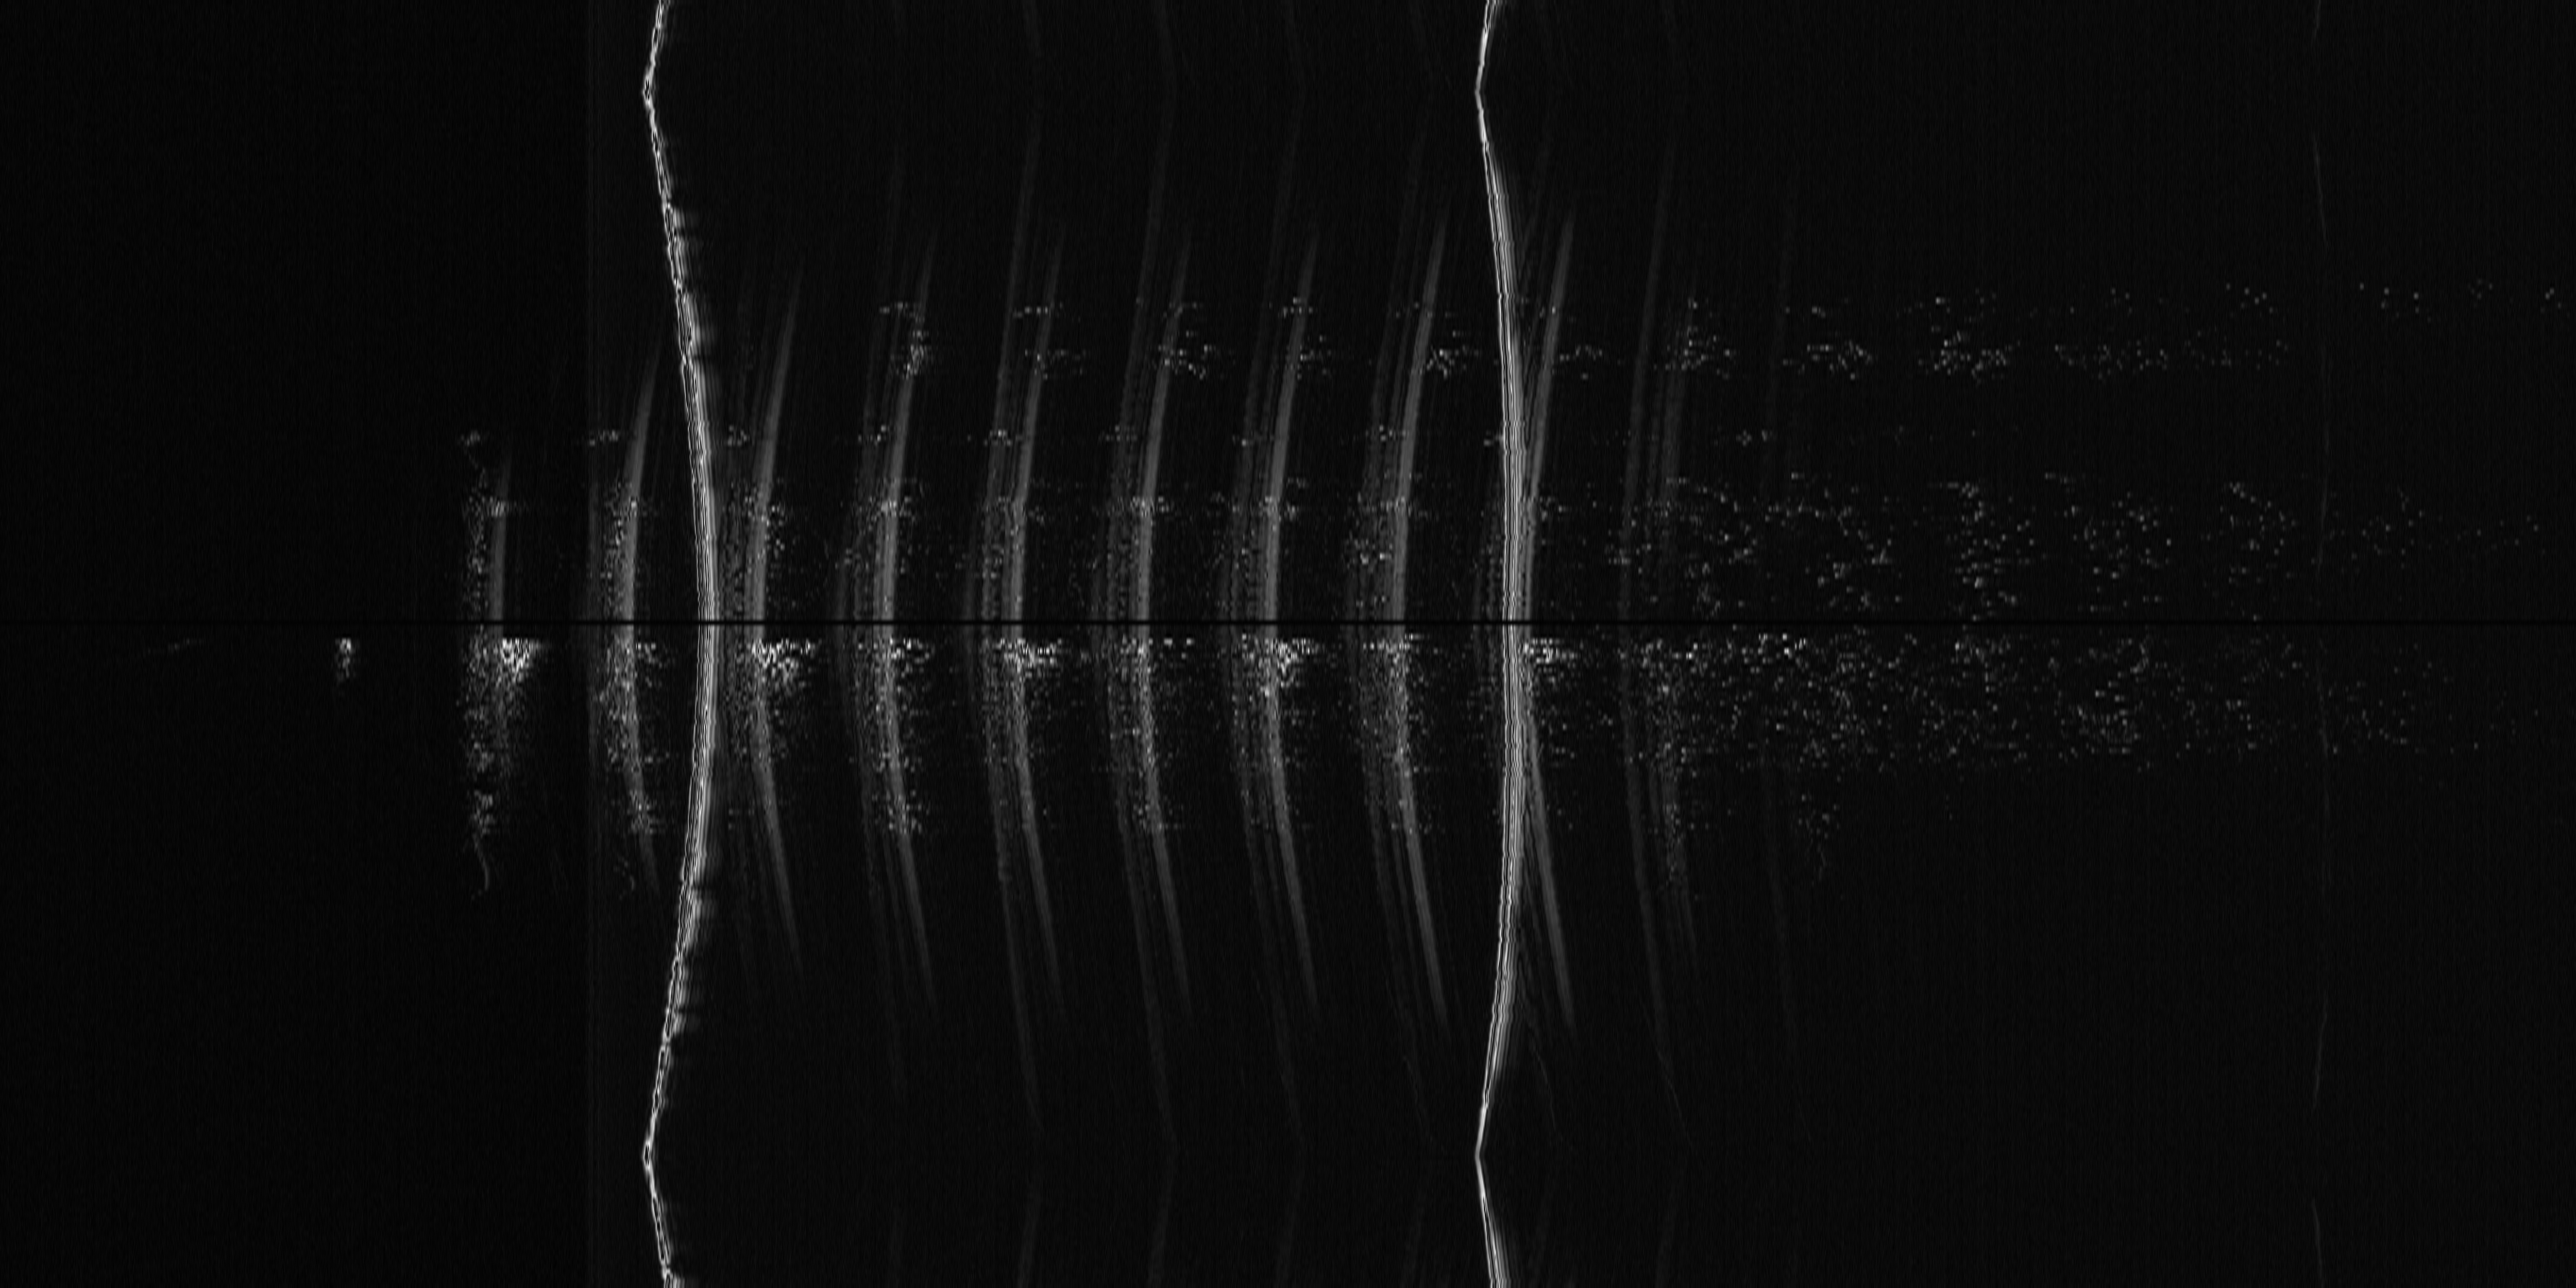
\includegraphics[width=0.75\textwidth]{C3water8500003.png}
     \caption{15db}
   \label{fig:water_cavitation_85}
\end{figure}


\Figref{water_cavitation_70} shows two plots.
The images are the Hilbert transform of the RF data along the A-lines obtained from the Cortex scanner.
I have informally called these B-mode images - but in reality I have done nothing other than  

The top image is generated when both the driving wave and the imaging waves are on.
The two lines are the front and rear of the Mylar film, as imaged by the high frequency wave.
The lower plot is the same sample but when just the imaging wave is on.


In the top plot one can see banded specks that coincide  with the passing  driving wave.  
The temporal interval between the bands is consistent with the frequency of the driving wave.
%These are cavitation signals - you cannot make out the direct transmit in the image.
These signals are not present when the driving wave is off. % indicating that the signals are short lived (i.e. less than a few milliseconds - the time between adjacent A-lines).

At 30db suppression  such signals are  common but by no mean ubiquitous.
Often such signals are present only  few A-lines (grouped together, as above), sometimes only for a single A-line in the image, and often no visible at all.
At greater suppression (i.e 32 db) you get such signals but with a lesser frequency,
at a lesser suppression they become more common.
The 30db signal has the property that you see  the bubbles at gains that  do not pick up the direct transmit.
This gives the images its `clean' appearance.

%In this document I give images for two pressures - the 30db suppression (\figref{water_cavitation_70}) and 15db suppression (\figref{water_cavitation_85}).
%I have images for pressures in between and either side, but the figures indicate what can and can't be done with the data, I think.

%\subsubsection{Interpretation of the results}

%\subsubsection{Quantifying Results}
%A question that has not already been discussed could be  ``at what pressure does the cavitation signal manifest''.

%The probabilistic nature of a cavitation is commonly overcome by asking for the pressure at which you 
%generate a cavitation event in  50\% of the A-lines.
%This approach was taken by Herbert\cite{Herbert2006} for the homogeneous nucleation of water.
%Indeed, Herbert generated the probability density as a function of pressure.%

%However, it must be remembered that I am not doing homogeneous nucleation - 
%the probability of a cavitation event is not a function of the water, 
%but a function of its cleanliness and the degree to which the water is degassed.
%So while I could plot a graph such as Herbert's, and quote a `threshold', I am not sure what this threshold would t%ell me?
%Furthermore - since I am not {\em generating} a bubble (I am making an existing pocket of gas visible) - 
%two separate A-lines are not independent. 
%This invalidates the approach, and so any threshold I quote (of uncertain meaning) would be of dubious validity.%

%\todo[inline]{I cannot think of other relevant questions that I could ask of my data?}


 \Figref{water_cavitation_85} plots the image that is obtained with a driving voltage that is 15db greater than in \Figref{water_cavitation_70}.
More regular banding is evident in addition to the more stochastic events observed before.

\subsubsection{Interpretation}

The regular banding in \figref{water_cavitation_85} is very stable.
It is present only when the driving wave is, increases in amplitude with the driving wave,
and is of the same wavelength as the driving wave.
The most natural interpretation is that this portion of the image is the 
direct transmit of the driving wave arriving on the imaging wave.

The signal from the direct transmit is useful because it indicates the sampling of the compression
and rarefaction cycles of the driving wave by the imaging wave.
While it must be remembered that the imaging transducer is filtering the frequencies of the actual received signals,
thereby distorting them in the image, 
the broad phase of the driving wave is nevertheless evident in \figref{water_cavitation_85},
with the bright pixels indicating a compression in the driving wave.

The bright and stochastic signals that are seen on top of the direct transmission 
are interpreted as resulting from bubbles in the solution.
It is seen that their greatest intensites come in at the beginning of the rarefaction phase of the driving wave - the rebound after the compression. 
The lack of coherence between adjacent alines indicate that the bubbles are short lived (milliseconds).
This is expected from the analysis of \chapref{nucleation}.

Both \figref{water_cavitation_70} and \figref{water_cavitation_85} were driven with a
10 cycle burst from the driving transducer.
In \figref{water_cavitation_85}, however, 16 bands can be counted in the signal.
This suggest that the generated bubble through for the duration of the driving pulse (microseconds)
and interacts with the ringdown of the transducer after its burst.
It suggests that the bubbles are not destroyed and reborn on every cycle of the driving wave.


\subsubsection{What remains ambiguous}
Unfortunately a number of questions are not answered by the \figref{water_cavitation_70}
and  \Figref{water_cavitation_85}.
\desc{
\item[The location of the scattering bubble(s):]
  The location of the bubble(s) within the sample is not clear in the experiment.
  The signal detected by the imaging wave could result from one bubble, 
  generating an acoustic output with every cycle of the driving wave.
  
  However, even if there is only one bubble,  there is no indication as to its location.
  It could be anywhere along the axis between the two transducers.
  The localisation of an interacting bubble id entirely based upon the
  driving wave being focused.
  In \figref{zAxis} it is seen that this gives quite a lot of scope for the location of the bubble.

  The excess pressure cannot be applied in this experiment to help determine the location of the bubble.
  This is because the because the imaging transducer is moving between alines.

  
  Alternatively, the generated signal could be a superposition from many bubbles,
  again not necessarily at the imaging depth of the high-frequency transducer. 
  However, \Figref{water_cavitation_70} does provide some evidence contrary to this at low pressures.
  The 'all or nothing' characteristic evident in that figure suggests that there are not many 
  bubbles contributing to the signal.
  
\item[The role, if any, of the imaging wave:]
  The more serious ambiguity concerns the role of the imaging wave.
  It is not clear as to whether the backscatter from the imaging wave is contributing to the images at all.

  If the signal is just forward scatter then the experiment is simply doing passive cavitation detection
  via an overly complicated harmonic imaging setup.
  In this case there is little relation to the computational analysis of \chapref{computations}
  and there is no new technology at work.
  It should also be said that if this is the case then we are also using the word cavitation in its loosest sense.
  We could not claim to be generating a bubble - the bubble probably does exist, but is just not visible at the pressures and frequencies used in the imaging setup.
  The result would then be ``If you use a sufficiently high pressure you can pulsate a small bubble  to generate higher-frequency harmonics''.

  If, on the other hand, the signal is a combination of forward-scatter and backscatter then it would be a very interesting result.  
  We need a way of separating out `interesting' backscatter from the dull forward scatter,
  an issue was discussed at length in \chapref{mechanisms}.
  The way to do this is to subtract an image generated when only the driving wave is present (providing the forward scatter and direct transmit)
  from an image containing both waves.
  Then you are left with the contribution from the imaging wave.
  However, this is impossible with the current experimental setup.
  Since the driving wave is further from the cofocus than the imaging wave,
  it must be the driving wave that fires first and triggers the experiment.
  Unfortunately the Cortex scanner cannot be triggered in this way.
  Additionally, the technique relies upon both repetitions imaging the same bubble.
  The pendulum motion of the Cortex scan had is also therefore  inappropriate.
}

 The problem with the preliminary setup, therefore,  is that it is impossible to distinguish an interesting result (the driving wave and imaging wave interacting)
 from a result that contributes very little (harmonic imaging).
 



\subsection{The final experimental design} \label{sec:exp:finalDesign}

To resolve this problem the imaging transducer needs to be able to be turned off.
 However, this is not easy to do with the Cortex.
 To answer these questions I need a pulse-receive system that lets me choose which transducer is off/on at any give time.

%<<<<<<< HEAD
% \section{Characterisation of the bubbly fluid}
  
% The characterisation of the nucleation sources within the water can be achieved indirectly
% using a method discussed in \secref{WE:characterisation}.  
%=======
%\section{Characterisation of the bubbly fluid}
%  
%The characterisation of the nucleation sources within the water can be achieved indirectly
%using a method discussed in \secref{WE:characterisation}.  
%>>>>>>> 061ae1ca44e322a36342ec8f9f946d2793a172c6

% \subsection{Density of Impurities and threshold}
% Argument from Herbert\cite{Herbert2006}.

% Let $dn/dP$ be distribution of impurities with threshold $P$.
% I.e. concentration of impurities with threshold between $P$ and $P+dP$ is $(dn/dP)dP$
% Cavititation probability when pressure reaches $\Pmin$ at the focus,
% \begin{align}
%   \sum\lr{\Pmin} = 1- \exp\lr{-\int_Vdr \int_{P(r)}^\Psat dP \frac{dn}{dP} }
% \end{align}
% $V$ is volume of the focal region

% Simplest distribution assumes all have the same threshold 
% \begin{align}
%   \frac{dn}{dP} = n_0 \delta(P-P_0)
% \end{align}
% Then 
% \begin{align}
%   \sum\lr{\Pmin} = 1- \exp\lr{-n_0 V(P<P_0|\Pmin)}
% \end{align}
% If spherical distribution so that 
% \begin{align}
%   P(r) = \Pmin \frac{\sin(kr)}{kr}
% \end{align}
% then
% \begin{align}
%   \sum\lr{\Pmin} = 1- \exp\lr{-n_0 4\pi r^3 /3}
% \end{align}
% which can be expressed in terms of power series of $\epsilon \equiv 1-P_0/\Pmin$.
% But this provides bad fit
% Herbert tries distribution:
% \begin{align}
% \frac{dn}{dP} = \frac{\alpha n_0}{\lr{P_2-P_1}^{\alpha}}\lr{P_2-P}^{\alpha-1}
% \end{align}
% which can be fit well.

% \subsection{Distribution of bubbles}

% Diffusion vs buyancy.

% \subsection{Boolean model}
% From Stoyan Stochastic geometry and its applications.

% Constructed with {\em germs} $x_n$ and the {\em primary grains}, $\Xi_n$, such that
% \begin{align}
%   \Xi = \bigcup_{n=1}^\infty \lr{\Xi_n + x_n} = \lr{\Xi_1 + x_1} \cup \lr{\Xi_2 + x_2} \cup\ldots .
% \end{align}
% With condtion that 
% \begin{align}
%   E(\nu_d(\Xi_0 \oplus K)) < \infty \text{ for all compact k}
% \end{align}
% $\Xi_0$ denotes a further random compact set of same distribution of $\Xi_n$ but independent of both of them and of the germ process $\Phi$.
% $\Xi$ is a {\em boolean model with primary grain } $\Xi_o$.

% Condition ensures finitely many of the grains $\Xi_n+x_n$ meet any given compact set,
% ensuring property of beiing a closed set is inherited by $\Xi$ from the primiary grains.
% A simpler but more restrictive condition is that 
% \begin{align}
%   E(R^d) < \infty
% \end{align}
% where $R$ is the radius of the ball circumscribing $\Xi_n$.

% The primary grains are here spheres of random radius, drawn from a distribution, $M$,
% the {\em mark distribution}.
% They are therefore convex.

% Not assumed to be much overlap,
% therefore considered as a point process, the Neyman-scott point process

% \subsubsection{Capacity Functional}
% Determined uniquely by the {\em capacity functional}, $T_\Xi$.

% \begin{align}
% T_\Xi (K) &= P(\Xi \cap K \text{ is not empty}) \\
% &= P(\Xi \cap K \ne 0)
% \end{align}
% for any compact K.

% From the Poisson assuption, 
% \begin{align}
%   T_\Xi (K) = 1 - \exp\lr{-\lambda E(\nu_d(\check{\Xi}_0 \oplus K))}
% \end{align}
% or 
% \begin{align}
%   T_\Xi (K) = 1 - \exp\lr{-\lambda E(\nu_d({\Xi}_0 \oplus\check K))}
% \end{align}
% and the proof is in Stoyan.

% Useful to intodcue 
% \begin{align}
%   \psi(K) = 0 \ln P(\Xi \cap K = \absurdity).
% \end{align}
% so that
% \begin{align}
%   \psi(K) = \lambda E(\nu_d(\Xi_0 \oplus \check K))
% \end{align}

% \subsection{Neyman-Scott Point Process}


% \subsubsection{Contact Distribution functions}
% {\em Contact distribution function} or {\em hit distrubution function}
% for a stationary random closed set $\Xi$ is defined by using a specified test set or structuring element $B$,
% a convex body of $R^d$ containing the origin $o$.
% Then the contact distribution function is defined as
% \begin{align}
%   H_B(r) = 1 - \frac{P(\Xi\cap rB = \absurdity)}{1-p}
% \end{align}
% for $r\ge 0$ and where $p$ is the volume fraction of $\Xi$.
% Since $B$ contains the origin, $\Xi\cap rB$ being empty implies that $\Xi$ does not conatin the origin. So the value of $H_B(r)$ is the conditional probablity that the parallele set of distance $r$ of $B$ makes contact with $\Xi$, conditional on $\Xi$ nt containing $o$.

% The sphecica contact ditribution may be interpreted as the distrubtion functionof distance from a point chosen randomly outside $\Xi$,
% measured to the nearest point $Xi$.  Hence, $H_s$ is the law of first contact.

% In general we have
% \begin{align}
%   H_B(r) = 1- \exp\lr{-\lambda\lr{E\lr{\nu_d \lr{\check \Xi_0 \oplus r B}}- E\lr{\nu_d{\Xi_0}}}}
% \end{align}
% for $r\ge 0$.

%  Let $\Xi_\ast$ be a primary grain chosen at random, the ``typical'' grain.
%  Let $x_\ast$ be the corresponding germ of the typical grain, $\Xi_\ast$ and let
%  \begin{align}
%    \Xi^\prime = \bigcup\left\{\Xi_i + x_i : x_i \ne x_\ast \right\}
%  \end{align}
%  be the union of the ramaining grains, then the following are of interest,
%  \begin{align}
%    p_o &= P(x_\ast \text{ is covered by $\Xi^\prime$}\\
%    p_G &= P(\Xi_\ast + x_\ast \text{ intersects $\Xi^\prime$}),\\
%    p_s &= \text{fraction of boundary of $\Xi_\ast$ which is covered by $Xi^\prime$}
%  \end{align}
%  Probabities satisfy
%  \begin{align}
%    p_0 &= p\\
%    p_G &= 1 - E\lr{\exp\lr{-\psi\lr{\Xi_0}}}\\
%    p_s &= p
%  \end{align}
%  for proofs see Stoyon.

% The number of isolated grains with germ pointst in a given compact set $K$ is 
% \begin{align}
%   \lambda \lr{1-p_G}\nu_d(K)
% \end{align}

% \subsubsection{Convex Grains}
% If $\Xi_0$ is isotropic and convex then $\psi(K)$ can be calculatd for convex $K$ by the generalised Steiner Formula,
% \begin{align}
%   \psi(K) = \lambda E(\nu_d(\Xi_0 \oplus \check K)) = \frac{\lambda}{b_d}\sum_{k=0}^d \twovec{d}{k}\bar W_k W_{d-k}(K)
% \end{align}
% Where $\bar W_k$ denotes the mean of the $k$th Mindowski function of $\Xi_0$,
% \begin{align}
%   \bar W_k = E(W_k(\Xi_0)) \text{ for $k = 1, \ldots, d$}
% \end{align}
% and $b_d$ is the volume of the $d$-dimensional unit ball.

% E.g. let $X_0$ be a sphere, $b(o,R)$ of random radius $R$ with $E(R^d) <\infty$.
% Then 
% \begin{align}
%   \psi(K)= \lambda(A(K) + U(K)E(R) + \pi E(R^2))
% \end{align}
% and if $d=3$ then
% \begin{align}
%   \psi(K) = \lambda\lr{  V(K) + S(K)E(R) + 2\pi \bar b(K) E(R^2) + \frac{4}{3} \pi E(R^3) }
% \end{align}

% \subsubsection{Contact Distribution Function}
% For convex structure We have
% \begin{align}
%   H_B(r) = 1 - \exp\lr{ -\frac{\lambda}{b_d}\sum_{k=1}^d\twovec{d}{k}r^k \bar W_k W_{d-k}(B)}
% \end{align}
% for $r\ge 0$.
% The $k=0$ term cancels with $-\lambda \bar W_0$ or $-\lambda E(\nu_d(\Xi_0))$ terms.

% If $d=3$ then
% \begin{align}
%   H_B(r) &= 1 - \exp\lr{-\lambda \lr{\frac{\bar S M(B)}{4\pi}r + \frac{\bar M S(B)}{4 \pi}r^2 + V(B) r^3 } }\\
%   &= 1 - \exp\lr{ -\frac{1}{1-V_V} \lr{ \frac{S_V M(B) }{4\pi}r + \frac{M_V^+S(B)}{4\pi}r^2 + N_V^+V(B)r^3  } }
% \end{align}
% for $r\ge 0$.
% N.B. The physical dimensionality of the $H_B(r)$ has to be noted.  See the book.

% Spherical Contact Distribution
% \begin{align}
%   H_s(r) = 1-\exp\lr{-\lambda \sum_{k=1}^d\twovec{d}{k} \bar W_kr^k}
% \end{align}
% for $r\ge0$.
% It is the distance to the nearest sphere from a point chosen at random but from outside one of the spheres.
% It is 
% \begin{align}
%    H_s(r) = 1-\exp\lr{-\frac{4}{3}\pi\lambda r\lr{3E(R^2) + 3r E(R) + r^2}}
% \end{align}

% Special cases
% Primary grains are random balls with radius $R$ and distribution function $F_R$ with
% \begin{align}
%   p = 1- \exp\lr{-\frac{4}{3}\lambda \pi E(R^3)}
% \end{align}
% \begin{align}
%   \lambda_1^{(3)} = \lambda \pi E(R^2)
% \end{align}
% \begin{align}
%   H_s(r) = 1 - \exp\lr{ -\lambda \pi r \lr{ 4 r E(R) + \frac{4r^2}{3} }  }
% \end{align}
% \begin{align}
%   C(r) = 2p - 1 + \lr{1-p}^2 \exp \lr{ \lambda \frac{4}{3}\pi \int_{r/2}^\infty x^3\lr{1-\frac{3r}{4x}+\frac{r^2}{16x^3}} dF_R(x)}
% \end{align}

% \subsection{Proximity of Bubbles}
% Are they likely to be interacting

% \subsection{Probability of a bubble in the imaging field of view}

% \subsection{Probability of a bubble in the Driving field of view}



% First, however, we motivate the use of tap water with a few examples of the nucleation images that can be generated.

%}







% \subsection{Generation of the two pulses}
% \subsubsection{Imaging wave}
% The imaging wave is generated from a custom ordered Panemetrics \unit{20}\mega\hertz\
% transducer.
% The pulse/receive electronics is controlled 
% with a \JsrUltrasonics \DPR500 dual pulser-receiver
% with a \RPL2 pulser-receiver.
% The imaging voltage was \unit{300}\volt\ and the combined imaging gain 
% of the pre-amplifier and \DPR500 was \unit{50}dB.
% To help reduce the contribution of the direct transmit/forward scatter of
% the driving wave, a high pass filter (-\unit{3}dB at \unit{7.5}\mega\hertz)
% was used.

% \subsubsection{Driving wave}
% The driving wave was generated from an  Analogic 2045 arbitrary waveform generator.
% The input voltage was a sinusoid of frequency \unit{0.5}\mega\hertz\ 
% truncated to be 10 cycles in duration. 
% The output of Analogic was input into a Tomco power-generator (gain of \unit{50}dB)
% which drove a \unit{0.5}\mega\hertz\ ... transducer.

% \subsubsection{Controlling the timing of the two waves}
% An Agilent  33220A is controlled by LAN connection.  Its role is trigged by the computer to produce a sine burst of 10 cycles.  The gate to the tomco and the analogic is conneted to the sync out.  The output is connected to the RF in on the Tomco

% The analogic is to provide a delayed pulse for the \DPR500.  The reason this pulser is used rather than the Thandars or the agilent is because it has a much faster clock.  The other generators are not usable because the gitter is of order 50ns  ruining the averages.  The gitter from the analogic is nearer 5-10ns.  Its output goes to trigger the scope and to the sunc of the \DPR500.  The scope is triggered from this input so that the time recorded is genuinly a pulse-echo-time.


% The \DPR500 is controlled via serial connection.  It controls the imaging spike.

% The scope is controlled by LAN. Waveforms are grabbed directly from the scope.


% %When imaged by the high-frequency wave the phase of the low frequency
% %wave will manifest itself as a function of depth.



% %The two pulses transducers need to have a common focus and we wish to
% %interrogate all phase relationships between the two waves.
% %This is most easily achieved by
% %In this experimental arrangement the firing of the two pulses is co-ordinated so that the waves meet at
% %their common focus at the same time.
% %As they pass through each other at twice the speed of sound the two waves will pass through all
% %possible phases.
% %When imaged by the high-frequency wave the phase of the low frequency
% %wave will manifest itself as a
% %function of depth.
% %(If this is not clear then \figref{pulses} in \secref{computational}
% %may help.) 



% %The limited bandwidth of the high-frequency transducer is relied upon
% %to filter out the direct transmit of the low-frequency wave.


% \subsection{The Experimental container}
% The experiment is carried out with a experimental chamber built by Mr Craig ...
% The dimensions are drawn in \figref{chamber_drawing}
% and a photo is seen in \figref{chamber_photo}.
% A water bath is provided for both the driving and imaging transducers,
% both such that the geometric focus is coincident in the middle of central,
% reaction chamber.
% the central chamber can be closed with a plastic acoustic medium.
% However,
% in this experiment no such division was made.


% \subsection{Summary of arrangement}
% The full arrangement is given in \figref{arrangement}.



% %\subsection{The characterisation of the nucleated bubbles}\label{sec:WE:characterisation}


% \subsection{The experimental volume}

% Beamplot goes here.

% \subsubsection{Generation of Bubbles}

% \subsubsection{Assumptions made}





%When I high frequency wave - the imaging wave -
%is incident 
%It does so indirectly.
%First, the 
%It was shown that when a bubble is shrunk, 
%even temporarily, 
%that the resonance frequency of the bubble increases.
%The bubble's response to a high frequency imaging wave can be tuned by varying the phase of% the bubble's cycle at which the bubble is incident.
%The phase of the bubble, in turn,
%may be controlled by a second, lower frequency wave.
%When the phase of the low frequency wave - the driving wave - 
%is such that the bubble is temporarily shrunk,
%the resonance frequency of the bubble temporarily increases.
%If a short high frequency pulse is incident on the b
%The bubble's response to a second, high frequency imaging wave can be tuned by varying the phase relationship between the two waves.




% \section{A motivating  example}\label{sec:WE:motivating_ex}

% \begin{figure}[t]%
%   \centering
%   \subfloat[1st pulse - 100]{
%     \label{fig:av:108:100_ex:first}
%     % GNUPLOT: LaTeX picture with Postscript
\begingroup
  \makeatletter
  \providecommand\color[2][]{%
    \GenericError{(gnuplot) \space\space\space\@spaces}{%
      Package color not loaded in conjunction with
      terminal option `colourtext'%
    }{See the gnuplot documentation for explanation.%
    }{Either use 'blacktext' in gnuplot or load the package
      color.sty in LaTeX.}%
    \renewcommand\color[2][]{}%
  }%
  \providecommand\includegraphics[2][]{%
    \GenericError{(gnuplot) \space\space\space\@spaces}{%
      Package graphicx or graphics not loaded%
    }{See the gnuplot documentation for explanation.%
    }{The gnuplot epslatex terminal needs graphicx.sty or graphics.sty.}%
    \renewcommand\includegraphics[2][]{}%
  }%
  \providecommand\rotatebox[2]{#2}%
  \@ifundefined{ifGPcolor}{%
    \newif\ifGPcolor
    \GPcolortrue
  }{}%
  \@ifundefined{ifGPblacktext}{%
    \newif\ifGPblacktext
    \GPblacktexttrue
  }{}%
  % define a \g@addto@macro without @ in the name:
  \let\gplgaddtomacro\g@addto@macro
  % define empty templates for all commands taking text:
  \gdef\gplbacktext{}%
  \gdef\gplfronttext{}%
  \makeatother
  \ifGPblacktext
    % no textcolor at all
    \def\colorrgb#1{}%
    \def\colorgray#1{}%
  \else
    % gray or color?
    \ifGPcolor
      \def\colorrgb#1{\color[rgb]{#1}}%
      \def\colorgray#1{\color[gray]{#1}}%
      \expandafter\def\csname LTw\endcsname{\color{white}}%
      \expandafter\def\csname LTb\endcsname{\color{black}}%
      \expandafter\def\csname LTa\endcsname{\color{black}}%
      \expandafter\def\csname LT0\endcsname{\color[rgb]{1,0,0}}%
      \expandafter\def\csname LT1\endcsname{\color[rgb]{0,1,0}}%
      \expandafter\def\csname LT2\endcsname{\color[rgb]{0,0,1}}%
      \expandafter\def\csname LT3\endcsname{\color[rgb]{1,0,1}}%
      \expandafter\def\csname LT4\endcsname{\color[rgb]{0,1,1}}%
      \expandafter\def\csname LT5\endcsname{\color[rgb]{1,1,0}}%
      \expandafter\def\csname LT6\endcsname{\color[rgb]{0,0,0}}%
      \expandafter\def\csname LT7\endcsname{\color[rgb]{1,0.3,0}}%
      \expandafter\def\csname LT8\endcsname{\color[rgb]{0.5,0.5,0.5}}%
    \else
      % gray
      \def\colorrgb#1{\color{black}}%
      \def\colorgray#1{\color[gray]{#1}}%
      \expandafter\def\csname LTw\endcsname{\color{white}}%
      \expandafter\def\csname LTb\endcsname{\color{black}}%
      \expandafter\def\csname LTa\endcsname{\color{black}}%
      \expandafter\def\csname LT0\endcsname{\color{black}}%
      \expandafter\def\csname LT1\endcsname{\color{black}}%
      \expandafter\def\csname LT2\endcsname{\color{black}}%
      \expandafter\def\csname LT3\endcsname{\color{black}}%
      \expandafter\def\csname LT4\endcsname{\color{black}}%
      \expandafter\def\csname LT5\endcsname{\color{black}}%
      \expandafter\def\csname LT6\endcsname{\color{black}}%
      \expandafter\def\csname LT7\endcsname{\color{black}}%
      \expandafter\def\csname LT8\endcsname{\color{black}}%
    \fi
  \fi
  \setlength{\unitlength}{0.0500bp}%
  \begin{picture}(2880.00,2520.00)%
    \gplgaddtomacro\gplbacktext{%
      \csname LTb\endcsname%
      \put(-119,782){\makebox(0,0)[r]{\strut{}-1}}%
      \put(-119,1040){\makebox(0,0)[r]{\strut{}-0.5}}%
      \put(-119,1298){\makebox(0,0)[r]{\strut{} 0}}%
      \put(-119,1556){\makebox(0,0)[r]{\strut{} 0.5}}%
      \put(-119,1814){\makebox(0,0)[r]{\strut{} 1}}%
      \put(-119,2072){\makebox(0,0)[r]{\strut{} 1.5}}%
      \put(-119,2330){\makebox(0,0)[r]{\strut{} 2}}%
      \put(13,484){\makebox(0,0){\strut{} 0}}%
      \put(421,484){\makebox(0,0){\strut{} 5}}%
      \put(828,484){\makebox(0,0){\strut{} 10}}%
      \put(1236,484){\makebox(0,0){\strut{} 15}}%
      \put(1643,484){\makebox(0,0){\strut{} 20}}%
      \put(2051,484){\makebox(0,0){\strut{} 25}}%
      \put(2458,484){\makebox(0,0){\strut{} 30}}%
      \put(2866,484){\makebox(0,0){\strut{} 35}}%
      \put(-889,1590){\rotatebox{-270}{\makebox(0,0){\strut{}voltage (V)}}}%
      \put(1439,154){\makebox(0,0){\strut{}time ($\mu$ s)}}%
    }%
    \gplgaddtomacro\gplfronttext{%
      \csname LTb\endcsname%
      \put(2381,2303){\makebox(0,0)[r]{\strut{}1-$\sigma$}}%
      \csname LTb\endcsname%
      \put(2381,2083){\makebox(0,0)[r]{\strut{}av.}}%
    }%
    \gplbacktext
    \put(0,0){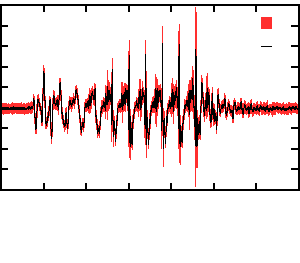
\includegraphics{voltage_0_108_gap_between_pulses_100_no_imaging_av_with_sd_means1_large}}%
    \gplfronttext
  \end{picture}%
\endgroup
}
%  \quad
%   \subfloat[2nd pulse - 100]{
%     \label{fig:av:108:100_ex:second}
%     % GNUPLOT: LaTeX picture with Postscript
\begingroup
  \makeatletter
  \providecommand\color[2][]{%
    \GenericError{(gnuplot) \space\space\space\@spaces}{%
      Package color not loaded in conjunction with
      terminal option `colourtext'%
    }{See the gnuplot documentation for explanation.%
    }{Either use 'blacktext' in gnuplot or load the package
      color.sty in LaTeX.}%
    \renewcommand\color[2][]{}%
  }%
  \providecommand\includegraphics[2][]{%
    \GenericError{(gnuplot) \space\space\space\@spaces}{%
      Package graphicx or graphics not loaded%
    }{See the gnuplot documentation for explanation.%
    }{The gnuplot epslatex terminal needs graphicx.sty or graphics.sty.}%
    \renewcommand\includegraphics[2][]{}%
  }%
  \providecommand\rotatebox[2]{#2}%
  \@ifundefined{ifGPcolor}{%
    \newif\ifGPcolor
    \GPcolortrue
  }{}%
  \@ifundefined{ifGPblacktext}{%
    \newif\ifGPblacktext
    \GPblacktexttrue
  }{}%
  % define a \g@addto@macro without @ in the name:
  \let\gplgaddtomacro\g@addto@macro
  % define empty templates for all commands taking text:
  \gdef\gplbacktext{}%
  \gdef\gplfronttext{}%
  \makeatother
  \ifGPblacktext
    % no textcolor at all
    \def\colorrgb#1{}%
    \def\colorgray#1{}%
  \else
    % gray or color?
    \ifGPcolor
      \def\colorrgb#1{\color[rgb]{#1}}%
      \def\colorgray#1{\color[gray]{#1}}%
      \expandafter\def\csname LTw\endcsname{\color{white}}%
      \expandafter\def\csname LTb\endcsname{\color{black}}%
      \expandafter\def\csname LTa\endcsname{\color{black}}%
      \expandafter\def\csname LT0\endcsname{\color[rgb]{1,0,0}}%
      \expandafter\def\csname LT1\endcsname{\color[rgb]{0,1,0}}%
      \expandafter\def\csname LT2\endcsname{\color[rgb]{0,0,1}}%
      \expandafter\def\csname LT3\endcsname{\color[rgb]{1,0,1}}%
      \expandafter\def\csname LT4\endcsname{\color[rgb]{0,1,1}}%
      \expandafter\def\csname LT5\endcsname{\color[rgb]{1,1,0}}%
      \expandafter\def\csname LT6\endcsname{\color[rgb]{0,0,0}}%
      \expandafter\def\csname LT7\endcsname{\color[rgb]{1,0.3,0}}%
      \expandafter\def\csname LT8\endcsname{\color[rgb]{0.5,0.5,0.5}}%
    \else
      % gray
      \def\colorrgb#1{\color{black}}%
      \def\colorgray#1{\color[gray]{#1}}%
      \expandafter\def\csname LTw\endcsname{\color{white}}%
      \expandafter\def\csname LTb\endcsname{\color{black}}%
      \expandafter\def\csname LTa\endcsname{\color{black}}%
      \expandafter\def\csname LT0\endcsname{\color{black}}%
      \expandafter\def\csname LT1\endcsname{\color{black}}%
      \expandafter\def\csname LT2\endcsname{\color{black}}%
      \expandafter\def\csname LT3\endcsname{\color{black}}%
      \expandafter\def\csname LT4\endcsname{\color{black}}%
      \expandafter\def\csname LT5\endcsname{\color{black}}%
      \expandafter\def\csname LT6\endcsname{\color{black}}%
      \expandafter\def\csname LT7\endcsname{\color{black}}%
      \expandafter\def\csname LT8\endcsname{\color{black}}%
    \fi
  \fi
  \setlength{\unitlength}{0.0500bp}%
  \begin{picture}(2880.00,2520.00)%
    \gplgaddtomacro\gplbacktext{%
      \csname LTb\endcsname%
      \put(-119,704){\makebox(0,0)[r]{\strut{}}}%
      \put(-119,926){\makebox(0,0)[r]{\strut{}}}%
      \put(-119,1147){\makebox(0,0)[r]{\strut{}}}%
      \put(-119,1369){\makebox(0,0)[r]{\strut{}}}%
      \put(-119,1590){\makebox(0,0)[r]{\strut{}}}%
      \put(-119,1812){\makebox(0,0)[r]{\strut{}}}%
      \put(-119,2033){\makebox(0,0)[r]{\strut{}}}%
      \put(-119,2255){\makebox(0,0)[r]{\strut{}}}%
      \put(-119,2476){\makebox(0,0)[r]{\strut{}}}%
      \put(13,484){\makebox(0,0){\strut{} 0}}%
      \put(421,484){\makebox(0,0){\strut{} 5}}%
      \put(828,484){\makebox(0,0){\strut{} 10}}%
      \put(1236,484){\makebox(0,0){\strut{} 15}}%
      \put(1643,484){\makebox(0,0){\strut{} 20}}%
      \put(2051,484){\makebox(0,0){\strut{} 25}}%
      \put(2458,484){\makebox(0,0){\strut{} 30}}%
      \put(2866,484){\makebox(0,0){\strut{} 35}}%
      \put(1439,154){\makebox(0,0){\strut{}time ($\mu$ s)}}%
    }%
    \gplgaddtomacro\gplfronttext{%
      \csname LTb\endcsname%
      \put(2381,2303){\makebox(0,0)[r]{\strut{}1-$\sigma$}}%
      \csname LTb\endcsname%
      \put(2381,2083){\makebox(0,0)[r]{\strut{}av.}}%
    }%
    \gplbacktext
    \put(0,0){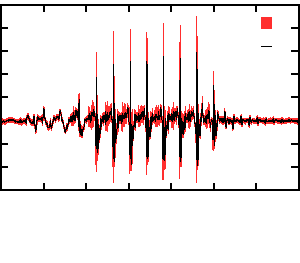
\includegraphics{voltage_0_108_gap_between_pulses_100_no_imaging_av_with_sd_means2_large}}%
    \gplfronttext
  \end{picture}%
\endgroup
}\\
%  \subfloat[1st pulse - 12000]{
%     \label{fig:av:108:12000_ex:first}
%     % GNUPLOT: LaTeX picture with Postscript
\begingroup
  \makeatletter
  \providecommand\color[2][]{%
    \GenericError{(gnuplot) \space\space\space\@spaces}{%
      Package color not loaded in conjunction with
      terminal option `colourtext'%
    }{See the gnuplot documentation for explanation.%
    }{Either use 'blacktext' in gnuplot or load the package
      color.sty in LaTeX.}%
    \renewcommand\color[2][]{}%
  }%
  \providecommand\includegraphics[2][]{%
    \GenericError{(gnuplot) \space\space\space\@spaces}{%
      Package graphicx or graphics not loaded%
    }{See the gnuplot documentation for explanation.%
    }{The gnuplot epslatex terminal needs graphicx.sty or graphics.sty.}%
    \renewcommand\includegraphics[2][]{}%
  }%
  \providecommand\rotatebox[2]{#2}%
  \@ifundefined{ifGPcolor}{%
    \newif\ifGPcolor
    \GPcolortrue
  }{}%
  \@ifundefined{ifGPblacktext}{%
    \newif\ifGPblacktext
    \GPblacktexttrue
  }{}%
  % define a \g@addto@macro without @ in the name:
  \let\gplgaddtomacro\g@addto@macro
  % define empty templates for all commands taking text:
  \gdef\gplbacktext{}%
  \gdef\gplfronttext{}%
  \makeatother
  \ifGPblacktext
    % no textcolor at all
    \def\colorrgb#1{}%
    \def\colorgray#1{}%
  \else
    % gray or color?
    \ifGPcolor
      \def\colorrgb#1{\color[rgb]{#1}}%
      \def\colorgray#1{\color[gray]{#1}}%
      \expandafter\def\csname LTw\endcsname{\color{white}}%
      \expandafter\def\csname LTb\endcsname{\color{black}}%
      \expandafter\def\csname LTa\endcsname{\color{black}}%
      \expandafter\def\csname LT0\endcsname{\color[rgb]{1,0,0}}%
      \expandafter\def\csname LT1\endcsname{\color[rgb]{0,1,0}}%
      \expandafter\def\csname LT2\endcsname{\color[rgb]{0,0,1}}%
      \expandafter\def\csname LT3\endcsname{\color[rgb]{1,0,1}}%
      \expandafter\def\csname LT4\endcsname{\color[rgb]{0,1,1}}%
      \expandafter\def\csname LT5\endcsname{\color[rgb]{1,1,0}}%
      \expandafter\def\csname LT6\endcsname{\color[rgb]{0,0,0}}%
      \expandafter\def\csname LT7\endcsname{\color[rgb]{1,0.3,0}}%
      \expandafter\def\csname LT8\endcsname{\color[rgb]{0.5,0.5,0.5}}%
    \else
      % gray
      \def\colorrgb#1{\color{black}}%
      \def\colorgray#1{\color[gray]{#1}}%
      \expandafter\def\csname LTw\endcsname{\color{white}}%
      \expandafter\def\csname LTb\endcsname{\color{black}}%
      \expandafter\def\csname LTa\endcsname{\color{black}}%
      \expandafter\def\csname LT0\endcsname{\color{black}}%
      \expandafter\def\csname LT1\endcsname{\color{black}}%
      \expandafter\def\csname LT2\endcsname{\color{black}}%
      \expandafter\def\csname LT3\endcsname{\color{black}}%
      \expandafter\def\csname LT4\endcsname{\color{black}}%
      \expandafter\def\csname LT5\endcsname{\color{black}}%
      \expandafter\def\csname LT6\endcsname{\color{black}}%
      \expandafter\def\csname LT7\endcsname{\color{black}}%
      \expandafter\def\csname LT8\endcsname{\color{black}}%
    \fi
  \fi
  \setlength{\unitlength}{0.0500bp}%
  \begin{picture}(2880.00,2520.00)%
    \gplgaddtomacro\gplbacktext{%
      \csname LTb\endcsname%
      \put(-119,782){\makebox(0,0)[r]{\strut{}-1}}%
      \put(-119,1040){\makebox(0,0)[r]{\strut{}-0.5}}%
      \put(-119,1298){\makebox(0,0)[r]{\strut{} 0}}%
      \put(-119,1556){\makebox(0,0)[r]{\strut{} 0.5}}%
      \put(-119,1814){\makebox(0,0)[r]{\strut{} 1}}%
      \put(-119,2072){\makebox(0,0)[r]{\strut{} 1.5}}%
      \put(-119,2330){\makebox(0,0)[r]{\strut{} 2}}%
      \put(13,484){\makebox(0,0){\strut{} 0}}%
      \put(421,484){\makebox(0,0){\strut{} 5}}%
      \put(828,484){\makebox(0,0){\strut{} 10}}%
      \put(1236,484){\makebox(0,0){\strut{} 15}}%
      \put(1643,484){\makebox(0,0){\strut{} 20}}%
      \put(2051,484){\makebox(0,0){\strut{} 25}}%
      \put(2458,484){\makebox(0,0){\strut{} 30}}%
      \put(2866,484){\makebox(0,0){\strut{} 35}}%
      \put(-889,1590){\rotatebox{-270}{\makebox(0,0){\strut{}voltage (V)}}}%
      \put(1439,154){\makebox(0,0){\strut{}time ($\mu$ s)}}%
    }%
    \gplgaddtomacro\gplfronttext{%
      \csname LTb\endcsname%
      \put(2381,2303){\makebox(0,0)[r]{\strut{}1-$\sigma$}}%
      \csname LTb\endcsname%
      \put(2381,2083){\makebox(0,0)[r]{\strut{}av.}}%
    }%
    \gplbacktext
    \put(0,0){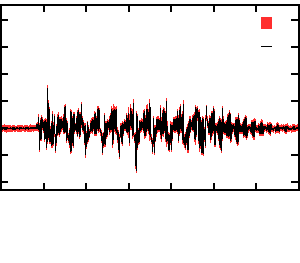
\includegraphics{voltage_0_108_gap_between_pulses_12000_no_imaging_av_with_sd_means1_large}}%
    \gplfronttext
  \end{picture}%
\endgroup
}
%  \quad
%   \subfloat[2nd pulse - 12000]{
%     \label{fig:av:108:12000_ex:second}
%     % GNUPLOT: LaTeX picture with Postscript
\begingroup
  \makeatletter
  \providecommand\color[2][]{%
    \GenericError{(gnuplot) \space\space\space\@spaces}{%
      Package color not loaded in conjunction with
      terminal option `colourtext'%
    }{See the gnuplot documentation for explanation.%
    }{Either use 'blacktext' in gnuplot or load the package
      color.sty in LaTeX.}%
    \renewcommand\color[2][]{}%
  }%
  \providecommand\includegraphics[2][]{%
    \GenericError{(gnuplot) \space\space\space\@spaces}{%
      Package graphicx or graphics not loaded%
    }{See the gnuplot documentation for explanation.%
    }{The gnuplot epslatex terminal needs graphicx.sty or graphics.sty.}%
    \renewcommand\includegraphics[2][]{}%
  }%
  \providecommand\rotatebox[2]{#2}%
  \@ifundefined{ifGPcolor}{%
    \newif\ifGPcolor
    \GPcolortrue
  }{}%
  \@ifundefined{ifGPblacktext}{%
    \newif\ifGPblacktext
    \GPblacktexttrue
  }{}%
  % define a \g@addto@macro without @ in the name:
  \let\gplgaddtomacro\g@addto@macro
  % define empty templates for all commands taking text:
  \gdef\gplbacktext{}%
  \gdef\gplfronttext{}%
  \makeatother
  \ifGPblacktext
    % no textcolor at all
    \def\colorrgb#1{}%
    \def\colorgray#1{}%
  \else
    % gray or color?
    \ifGPcolor
      \def\colorrgb#1{\color[rgb]{#1}}%
      \def\colorgray#1{\color[gray]{#1}}%
      \expandafter\def\csname LTw\endcsname{\color{white}}%
      \expandafter\def\csname LTb\endcsname{\color{black}}%
      \expandafter\def\csname LTa\endcsname{\color{black}}%
      \expandafter\def\csname LT0\endcsname{\color[rgb]{1,0,0}}%
      \expandafter\def\csname LT1\endcsname{\color[rgb]{0,1,0}}%
      \expandafter\def\csname LT2\endcsname{\color[rgb]{0,0,1}}%
      \expandafter\def\csname LT3\endcsname{\color[rgb]{1,0,1}}%
      \expandafter\def\csname LT4\endcsname{\color[rgb]{0,1,1}}%
      \expandafter\def\csname LT5\endcsname{\color[rgb]{1,1,0}}%
      \expandafter\def\csname LT6\endcsname{\color[rgb]{0,0,0}}%
      \expandafter\def\csname LT7\endcsname{\color[rgb]{1,0.3,0}}%
      \expandafter\def\csname LT8\endcsname{\color[rgb]{0.5,0.5,0.5}}%
    \else
      % gray
      \def\colorrgb#1{\color{black}}%
      \def\colorgray#1{\color[gray]{#1}}%
      \expandafter\def\csname LTw\endcsname{\color{white}}%
      \expandafter\def\csname LTb\endcsname{\color{black}}%
      \expandafter\def\csname LTa\endcsname{\color{black}}%
      \expandafter\def\csname LT0\endcsname{\color{black}}%
      \expandafter\def\csname LT1\endcsname{\color{black}}%
      \expandafter\def\csname LT2\endcsname{\color{black}}%
      \expandafter\def\csname LT3\endcsname{\color{black}}%
      \expandafter\def\csname LT4\endcsname{\color{black}}%
      \expandafter\def\csname LT5\endcsname{\color{black}}%
      \expandafter\def\csname LT6\endcsname{\color{black}}%
      \expandafter\def\csname LT7\endcsname{\color{black}}%
      \expandafter\def\csname LT8\endcsname{\color{black}}%
    \fi
  \fi
  \setlength{\unitlength}{0.0500bp}%
  \begin{picture}(2880.00,2520.00)%
    \gplgaddtomacro\gplbacktext{%
      \csname LTb\endcsname%
      \put(-119,782){\makebox(0,0)[r]{\strut{}}}%
      \put(-119,1040){\makebox(0,0)[r]{\strut{}}}%
      \put(-119,1298){\makebox(0,0)[r]{\strut{}}}%
      \put(-119,1556){\makebox(0,0)[r]{\strut{}}}%
      \put(-119,1814){\makebox(0,0)[r]{\strut{}}}%
      \put(-119,2072){\makebox(0,0)[r]{\strut{}}}%
      \put(-119,2330){\makebox(0,0)[r]{\strut{}}}%
      \put(13,484){\makebox(0,0){\strut{} 0}}%
      \put(421,484){\makebox(0,0){\strut{} 5}}%
      \put(828,484){\makebox(0,0){\strut{} 10}}%
      \put(1236,484){\makebox(0,0){\strut{} 15}}%
      \put(1643,484){\makebox(0,0){\strut{} 20}}%
      \put(2051,484){\makebox(0,0){\strut{} 25}}%
      \put(2458,484){\makebox(0,0){\strut{} 30}}%
      \put(2866,484){\makebox(0,0){\strut{} 35}}%
      \put(1439,154){\makebox(0,0){\strut{}time ($\mu$ s)}}%
    }%
    \gplgaddtomacro\gplfronttext{%
      \csname LTb\endcsname%
      \put(2381,2303){\makebox(0,0)[r]{\strut{}1-$\sigma$}}%
      \csname LTb\endcsname%
      \put(2381,2083){\makebox(0,0)[r]{\strut{}av.}}%
    }%
    \gplbacktext
    \put(0,0){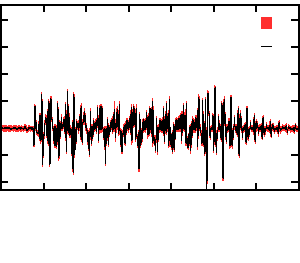
\includegraphics{voltage_0_108_gap_between_pulses_12000_no_imaging_av_with_sd_means2_large}}%
    \gplfronttext
  \end{picture}%
\endgroup
}\\
%   \subfloat[2nd pulse - 12000]{
%     \label{fig:av:108:12000_ex:sub}
%     % GNUPLOT: LaTeX picture with Postscript
\begingroup
  \makeatletter
  \providecommand\color[2][]{%
    \GenericError{(gnuplot) \space\space\space\@spaces}{%
      Package color not loaded in conjunction with
      terminal option `colourtext'%
    }{See the gnuplot documentation for explanation.%
    }{Either use 'blacktext' in gnuplot or load the package
      color.sty in LaTeX.}%
    \renewcommand\color[2][]{}%
  }%
  \providecommand\includegraphics[2][]{%
    \GenericError{(gnuplot) \space\space\space\@spaces}{%
      Package graphicx or graphics not loaded%
    }{See the gnuplot documentation for explanation.%
    }{The gnuplot epslatex terminal needs graphicx.sty or graphics.sty.}%
    \renewcommand\includegraphics[2][]{}%
  }%
  \providecommand\rotatebox[2]{#2}%
  \@ifundefined{ifGPcolor}{%
    \newif\ifGPcolor
    \GPcolortrue
  }{}%
  \@ifundefined{ifGPblacktext}{%
    \newif\ifGPblacktext
    \GPblacktexttrue
  }{}%
  % define a \g@addto@macro without @ in the name:
  \let\gplgaddtomacro\g@addto@macro
  % define empty templates for all commands taking text:
  \gdef\gplbacktext{}%
  \gdef\gplfronttext{}%
  \makeatother
  \ifGPblacktext
    % no textcolor at all
    \def\colorrgb#1{}%
    \def\colorgray#1{}%
  \else
    % gray or color?
    \ifGPcolor
      \def\colorrgb#1{\color[rgb]{#1}}%
      \def\colorgray#1{\color[gray]{#1}}%
      \expandafter\def\csname LTw\endcsname{\color{white}}%
      \expandafter\def\csname LTb\endcsname{\color{black}}%
      \expandafter\def\csname LTa\endcsname{\color{black}}%
      \expandafter\def\csname LT0\endcsname{\color[rgb]{1,0,0}}%
      \expandafter\def\csname LT1\endcsname{\color[rgb]{0,1,0}}%
      \expandafter\def\csname LT2\endcsname{\color[rgb]{0,0,1}}%
      \expandafter\def\csname LT3\endcsname{\color[rgb]{1,0,1}}%
      \expandafter\def\csname LT4\endcsname{\color[rgb]{0,1,1}}%
      \expandafter\def\csname LT5\endcsname{\color[rgb]{1,1,0}}%
      \expandafter\def\csname LT6\endcsname{\color[rgb]{0,0,0}}%
      \expandafter\def\csname LT7\endcsname{\color[rgb]{1,0.3,0}}%
      \expandafter\def\csname LT8\endcsname{\color[rgb]{0.5,0.5,0.5}}%
    \else
      % gray
      \def\colorrgb#1{\color{black}}%
      \def\colorgray#1{\color[gray]{#1}}%
      \expandafter\def\csname LTw\endcsname{\color{white}}%
      \expandafter\def\csname LTb\endcsname{\color{black}}%
      \expandafter\def\csname LTa\endcsname{\color{black}}%
      \expandafter\def\csname LT0\endcsname{\color{black}}%
      \expandafter\def\csname LT1\endcsname{\color{black}}%
      \expandafter\def\csname LT2\endcsname{\color{black}}%
      \expandafter\def\csname LT3\endcsname{\color{black}}%
      \expandafter\def\csname LT4\endcsname{\color{black}}%
      \expandafter\def\csname LT5\endcsname{\color{black}}%
      \expandafter\def\csname LT6\endcsname{\color{black}}%
      \expandafter\def\csname LT7\endcsname{\color{black}}%
      \expandafter\def\csname LT8\endcsname{\color{black}}%
    \fi
  \fi
  \setlength{\unitlength}{0.0500bp}%
  \begin{picture}(2880.00,2520.00)%
    \gplgaddtomacro\gplbacktext{%
      \csname LTb\endcsname%
      \put(-119,782){\makebox(0,0)[r]{\strut{}-1}}%
      \put(-119,1040){\makebox(0,0)[r]{\strut{}-0.5}}%
      \put(-119,1298){\makebox(0,0)[r]{\strut{} 0}}%
      \put(-119,1556){\makebox(0,0)[r]{\strut{} 0.5}}%
      \put(-119,1814){\makebox(0,0)[r]{\strut{} 1}}%
      \put(-119,2072){\makebox(0,0)[r]{\strut{} 1.5}}%
      \put(-119,2330){\makebox(0,0)[r]{\strut{} 2}}%
      \put(13,484){\makebox(0,0){\strut{} 0}}%
      \put(421,484){\makebox(0,0){\strut{} 5}}%
      \put(828,484){\makebox(0,0){\strut{} 10}}%
      \put(1236,484){\makebox(0,0){\strut{} 15}}%
      \put(1643,484){\makebox(0,0){\strut{} 20}}%
      \put(2051,484){\makebox(0,0){\strut{} 25}}%
      \put(2458,484){\makebox(0,0){\strut{} 30}}%
      \put(2866,484){\makebox(0,0){\strut{} 35}}%
      \put(-889,1590){\rotatebox{-270}{\makebox(0,0){\strut{}voltage (V)}}}%
      \put(1439,154){\makebox(0,0){\strut{}time ($\mu$ s)}}%
    }%
    \gplgaddtomacro\gplfronttext{%
      \csname LTb\endcsname%
      \put(2381,2303){\makebox(0,0)[r]{\strut{}1-$\sigma$}}%
      \csname LTb\endcsname%
      \put(2381,2083){\makebox(0,0)[r]{\strut{}av.}}%
    }%
    \gplbacktext
    \put(0,0){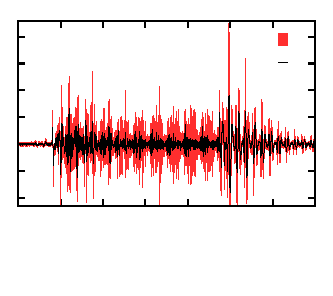
\includegraphics{voltage_0_108_gap_between_pulses_12000_no_imaging_av_with_sd_means_sub_large}}%
    \gplfronttext
  \end{picture}%
\endgroup
}\\
%   \caption{
%     The pressure received  by the imaging transducer when the driving wave is on but the imaging wave is off (receive-only).
%     The second pulse \subref{fig:av:108:100:second} is received \unit{100}\micro\second\ after the first \subref{fig:av:108:100:first}.
%     Each image is the average of 49 images, the first standard-deviation error bars are indicated.
%   }
%   \label{fig:av:108:100_ex}
% \end{figure}



% %\Figref{av:108:1000_ex:first} illustrates 

% To motivate the use of water as a the cavitating medium, 
% we illustrate a preliminary experiment that demonstrates the signal recieved by the high frequency transducer.
% \Figref{av:108:1000} shows the pressure received by the imaging transducer when the driving wave pressure is 0.108V at the focus.

% That a bubble is actually created is illustrated in 

% Need to demonstrate bubble.
% need to demonstrate nucleation threshold.
% need to demonstrate 

% %
% %Is it a bubble?
% %
% %Qualitatively the image is similar to those generated by the computer model.
% %A more detailed comparison on these lines will happen in \chapref{infer_model}.




% \nlist{
% \item homogeneity of bubble motes
% }




%In order to line with the goal of imaging an extravascular bubble,
%we focus in this chapter on imaging sub-micron bubbles 
%that have been pulled into solution with a low-frequency cavitating wave.
%This forces the experimental proceedure to 
%examine the major practical difficulty encountered when imaging with two ultrasound waves:
%the removal of the  bubble's high frequency response to the cavitating wave.
%As was shown in \chapref{mechanisms},
%if the driving wave is of sufficient pressure \todo{make this more precise}
%it will cause bubble to undergo an callapse with every cycle,
%each of which  can be detected by the imaging trasducer.
%This destroys the spatitial resolution of the image,
%for the bubble's temporal resolution is equal to the  duration of the low-frequeny pulse,
%rather than that of the much shorter imaging pulse.
%A method of overcoming this problem is to repeat the driving pulse,
%but this time without the imaging wave.
%By subtracting the response to the driving pulse alone,
%from the response when both waves are present,
%then the influence of the imagaging wave can be determined.
%This method propted the definition of {\em excess scattering cross section},
%given by \eqnref{excessI} on page \pageref{eqn:excessI}.
%This double-pulse method is explored in \secref{WE:method}.



%For a contrast agent to leave th
%In \chapref{introduction} \todo{check location of this} it was seen
%that if a contrast agent is to leave the blood,
%then its size is constrained to be smaller than approximatley 
%that even if a bubble contrast agent  that bubbles that are generated from a contrast agent that are able to leave the blood



%Generating a bubble with an acoustic pulse enables
%a bubble to be created and then imaged within a microsecond timeframe.
%This solves a major difficulty in the generation of small microbubbles:
%their ...\todo{get this number} lifespace.

%Reintroduce problem to solve,
%imaging a cavitated bubble





%\Chapref{mechanisms} investigated, with a computational model,
%how two ultrasound waves may be used 
%The generation and the imaging of a bubble places different requirements on an ultrasound pulse.

%\ilist{
%  \item the low frequencies and long pulses required for generating a bubble lead to poor resolution 
%when used for imaging;
%\item the size of the generated bubble is, in general,
%such that its resonance frequency is a poor match to the generating wave,
%which means that the bubble's response is sub-optimal,
%\item the 
%}
%the low frequencies and long pulses required for generating a bubble lead to poor resolution 
%when used for imaging;
%he size of the generated bubble is, in general,
%such that its resonance frequency is a poor match to the generating wave,
%which means that the bubble's response is sub-optimal;
%the high pressures used in the generating wave 


%The prediction of \chapref{mechanisms} requires two waves

%that the scattering of a bubble in response a high frequency wave
%can be modulated by the pulsations induced in the model with a second wave.

%When the driving wave shrinks the bubble, the resonance frequency temporarily increases.
%If the new resonance frequency is closer to that of the imaging wave, then the scattering increases.
%Otherwise it decreases.


%The principle difficulty in doing this is separating the influence of the imaging wave from 
%the scatter generated from the driving wave alone.
%To do so, as was discussed in \chapref{mechanisms},
%two pulses need to be taken, one with and one without the imaging wave.


%This chapter analyses the results of the experiment outlined int  whether the driving  wave influences the back-scatter from an imaging wave in the predicted manner.


%To determine the influence of the high frequency wave 
%on a bubble pulsating to a dual frequency wave,
%the influence 

%\Chapref{mechanisms} described a method of determining whether the scattering of a high frequency wave
%can be altered by the pulsations induced by  a lower frequency wave.
%Two pulses were required, 
%one comprising of low frequency and high frequency components,
%the other comprising of just low frequency components.
%In this way the unperturbed-forward scatter from the low frequency wave could be subtracted out, 
%leaving behind the scatter that is caused by the high frequency wave.

%However, using two pulses causes its own problems,
%for it is difficult to guarenee that the pulses are independant of one-another.
%A pulsating bubble can grow (rectified diffusion),
%can dissolve away or can burst into many smaller bubbles. 
%Additionally,
%even if 
%To generate a bubble, low frequencies and high pressures are required,
%parameters that are poor for imaging.


%There are two regimes where the tuning of the 
%is no
%The ability to tune the bubble's resonance frequency is not the only 
%use of theThe influence of the the low frequency wave is not only interesting because
%it allows the resonance frequency of the bubble to be tuned.



%To carry out such an experiment, however,
%requires a source of bubbles.


%Small bubbles. High pressures.



%\section{Discussion} \label{sec:WE:discussion}



%\Chapref{mechanisms} described a method of determining whether the scattering of a high frequency wave
%can be altered by the pulsations induced by  a lower frequency wave.
%Two pulses were required, 
%one comprising of low frequency and high frequency components,
%the other comprising of just low frequency components.
%In this way the unperturbed-forward scatter from the low frequency wave could be subtracted out, 
%leaving behind the scatter that is caused by the high frequency wave.

%This chapter gives two representative images at two different pressures for the cavitation of water.
%The issues in interpreting these images are then discussed.
%Without an interpretation, I do not believe we can say whether the images presented are novel or not, 
%even in terms of a balance of evidence.

%The images are Hilbert transformed data from the Cortex scanner.
%I have informally called these B-mode images - but in reality I have done nothing other than  Hilbert transform the RF data along A-lines.


% \todo[inline]{The following text has been taken from previous reports.
% The summary of this introduction has mostly been written in the introduction of \chapref{experimental_method},
% so this introduction can be skipped.
% I keep it here for the time being in case the structure enabled by \chapref{experimental_method} is not used,
% in which case this introduction will probably be required.
% }


% The main experimental parameters that are 
% subject to our control are:
% \nlist{
%   \item
%     The relative phase between the low-frequency and imaging wave.
%   \item
%     The pressures of the two waves.
%   \item
%     The frequencies of the two waves.
%   \item
%     The pulse-length of the two waves.
% }
% All variables other than the pulse length were investigated computationally in  \chapref{mechanisms}


% The first of these is well sampled by  virtue of the experimental
% setup.
% The two waves pass through each-other and so in {\em every} image {\em
%   all}
% phases between the two waves will be sampled.

% Sampling the pressure of the low-frequency wave is also
% straight-forward.
% A wide range of driving pulses are chosen to vary the peak pressure
% at the focus.
% In addition, since an 2D image is formed, 
% the spatially varying pressure field of the low frequency wave 
% will be imaged in  {\em every } image.
% The pressure of the imaging wave is much harder to control,
% for it is controlled internally by the scanner.
% %Indeed, it would be helpful to turn the imaging wave off altogether.
% %This cannot be achieved without modifying the scanner, however.
% The pressure ranges experimented with range from 0 through to $>1$ MPa
% peak-negative.

% Likewise, by choosing different  transducer, a range of
% frequencies  can be used for the two waves.
% Although our choice is not completely free.
% The high frequency pulse ideally should last for only a small fraction
% of the period of the low frequency wave.
% In addition, 
% when the difference in frequency between the low and high frequency transducers
% becomes small the direct transmission of sound between the transducer's
% becomes a problem for the anti-parallel setup of the transducers.
% Imaging frequencies of between 7.5 and 20 MHz have been tried, 
% along with low-frequency waves of between 0.5 and 2 MHz.
% The results presented here were used a 0.5 MHz low frequency wave and
% a 20 MHz imaging wave, unless otherwise stated.

% The pulse length of the imaging wave should be short, 
% although when imaging is achieved with a scanner, such as the cortex,
% then this parameter cannot be changed.
% The pulse length of the low frequency transducer is readily set.
% To avoid bubbles growing (by rectified diffusion), fusing (by Bjerknes
% forces) and collapsing (by instabilities in the oscillations) the low-frequency
% pulse should also be short.
% However, to reduce forward transmission the  frequency output of the
% low frequency wave should not be 
% too broad-band.
% 10 cycles is used in these experiments.

% The size of the bubbles/droplets is not simple to control.
% In general a fairly broad-range of sizes is present, even for the
% commercial agents,
% although one of the advantages of using commercially available
% contrast agents are that their size have been well studied.
% It is not possible to directly size the bubbles formed in cavitation,
% even though this is of interest.
% This is because the bubbles are too short lived.
% Finally, 
% sizing the perfluoropentane emulsion is also hard.
% This is because perfluoropentane is a transparent fluid with
% essentially the same refractive index as water,
% and so optical sizing becomes hard.
% The best that can be done so far is to bound the size distributions by
% passing the emulsion though a filter.
% For other reasons it is desirable to attach a fluorescent
% marker to the emulsion, but as a bonus this should help size the
% droplets.




% \subsection{Cavitated Water}\label{sec:water_vapourisation}

% I have done cavitation experiments for lots of different driving pressures.
% These pressures are recorded in my notes in terms of the number of decibels that the electric signal to the amplifier was suppressed.
% Since the number of pressures tried was great, and since beam plots takes a long time,
% I have only done axial  beamplots for 4 of the pressures tried.

% \Figref{water_cavitation_70} indicates the cavitation events recorded at 30db suppression.
% I have the (geometric) axial beam plot for this pressure.
% I have the code to process the beamplot data (to indicate the pressure at each location in th image, 
% although this code is untested and I haven't done the final step to actually draw it on the data.
% This final step - all being well- shouldn't take long. 
% It is my task, I think, for as soon as this document is finished.

% In this document I give images for two pressures - the 30db suppression (\figref{water_cavitation_70}) and 15db suppression (\figref{water_cavitation_85}).
% I have images for pressures in between and either side, but the figures indicate what can and can't be done with the data, I think.


% \begin{figure}[h]
%      \centering
%           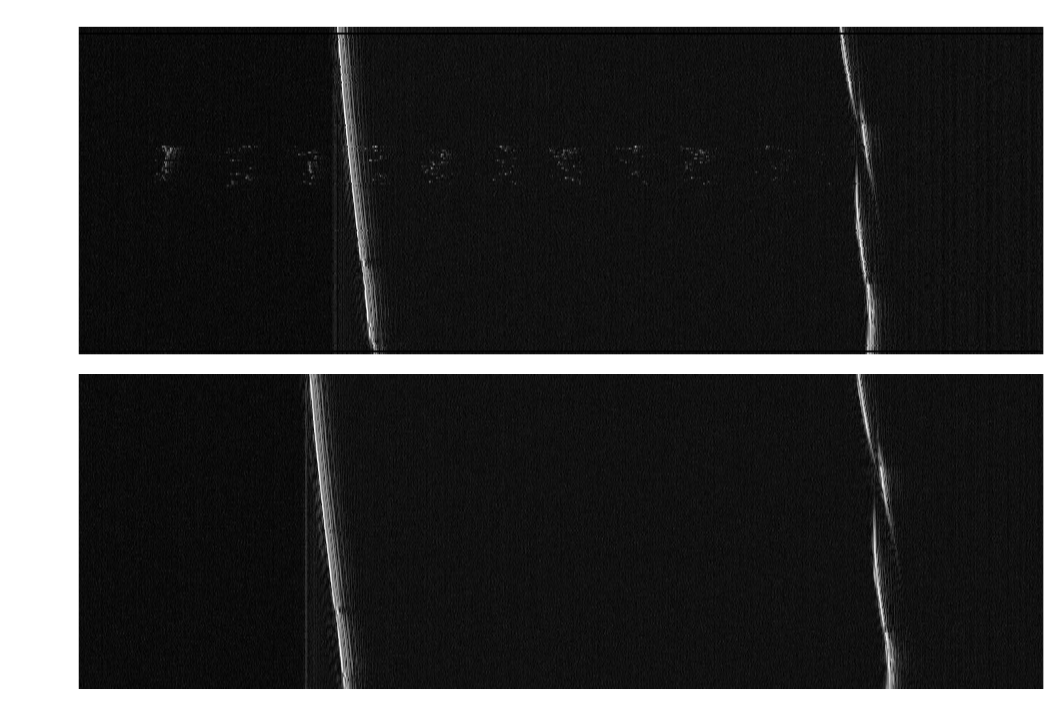
\includegraphics[width=0.8\textwidth]{rotterdam_02_water.png}
%      \caption{30db}
%    \label{fig:water_cavitation_70}
% \end{figure}

% \subsection{\Figref{water_cavitation_70}}
% \subsubsection{General discussion of the image}
% \Figref{water_cavitation_70} shows two plots.
% Above is the B-mode for when both the driving wave and the imaging wave is on.
% The two lines are the front and rear of the sample holder.
% The lower plot is the same sample but when just the imaging wave is on.

% In the top plot you can see banded specks that indicate the passage of the driving wave.  
% %These are cavitation signals - you cannot make out the direct transmit in the image.
% These signals are not present when the driving wave is off. % indicating that the signals are short lived (i.e. less than a few milliseconds - the time between adjacent A-lines).

% At 30db suppression  such signals are fairly common but by no mean ubiquitous.
% Often you get such signals only on a few A-lines (grouped together, as above) - sometimes only on 1 A-line - and often no signal at all.
% At greater suppression (i.e 32 db) you get such signals but with much lesser frequency, maybe signal on some A-lines once in every 5 or 6 frames.
% At lesser suppression they become more common.
% The 30db signal has the property that you see  the bubbles at gains that  do not pick up the direct transmit.
% This gives the images its `clean' appearance.

% \subsubsection{Interpretation of the results}

% \subsubsection{Quantifying Results}
% A question that has not already been discussed could be  ``at what pressure does the cavitation signal manifest''.

% The probabilistic nature of a cavitation is commonly overcome by asking for the pressure at which you 
% generate a cavitation event in  50\% of the A-lines.
% This approach was taken by Herbert\cite{Herbert2006} for the homogeneous nucleation of water.
% Indeed, Herbert generated the probability density as a function of pressure.

% However, it must be remembered that I am not doing homogeneous nucleation - 
% the probability of a cavitation event is not a function of the water, 
% but a function of its cleanliness and the degree to which the water is degassed.
% So while I could plot a graph such as Herbert's, and quote a `threshold', I am not sure what this threshold would tell me?
% Furthermore - since I am not {\em generating} a bubble (I am making an existing pocket of gas visible) - 
% two separate A-lines are not independent. 
% This invalidates the approach, and so any threshold I quote (of uncertain meaning) would be of dubious validity.

% \todo[inline]{I cannot think of other relevant questions that I could ask of my data?}


% \begin{figure}[h]
%      \centering
%           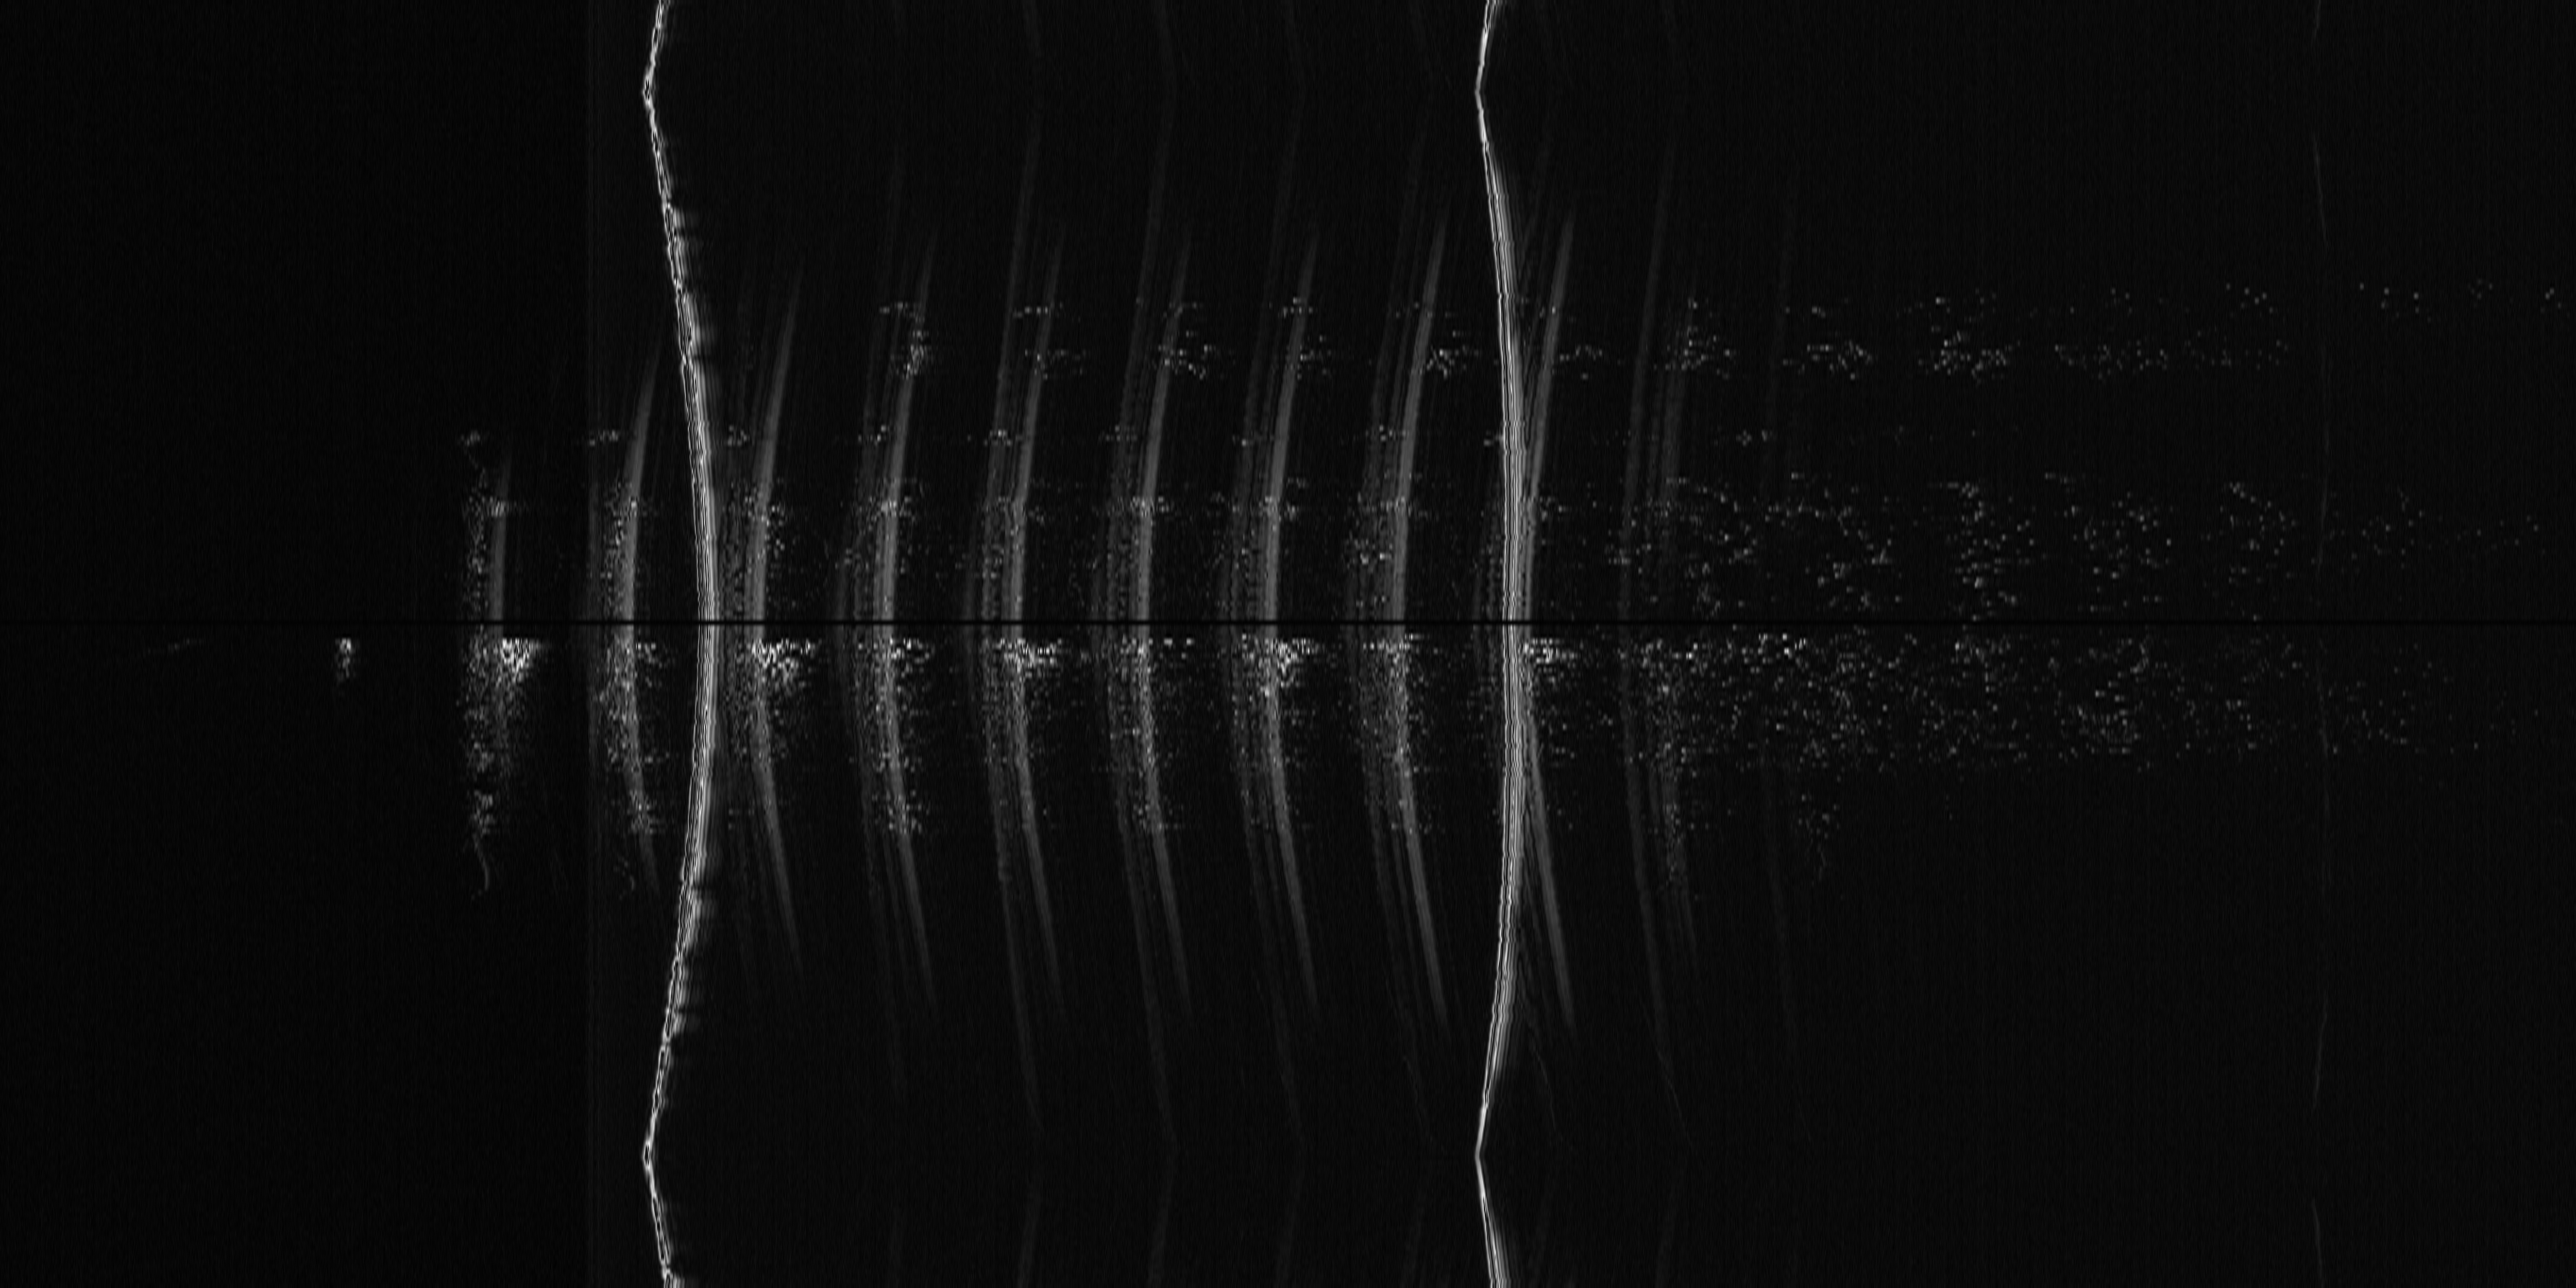
\includegraphics[width=0.8\textwidth]{C3water8500003.png}
%      \caption{15db}
%    \label{fig:water_cavitation_85}
% \end{figure}


% \subsection{\Figref{water_cavitation_85}}
% \subsubsection{General discussion of the image}
% The driving wave to \Figref{water_cavitation_85} has an applied voltage that is 15db greater than in \Figref{water_cavitation_70}.
% You can clearly see the forward transmit, and various cavitation events throughout the B-mode image.

% \subsubsection{The long tail of the image}
% The problems in with the interpretation of this image are similar to the previous image (with the same solutions).
% However, I include this image as I would like to draw your attention to what is in this image which is not in the previous.
% In \figref{water_cavitation_85} I can count 16 bands in the signal, whereas in \figref{water_cavitation_70} I can count 10, possibly 11.
% In both cases the signals were generated with a 10 electronic cycles. 
% The difference between the two is presumably the degree of ringing in the driving transducer after the power has been turned off.
% I have not done a beamplot for this pressure (John became a bit nervous about the cavitation events on the hydrophone).
% However, the fact that you can see banding well after the signal finished suggests 
% that you may see a response from the bubble even when the pressures from the driving transducer
% are much reduced.

% In these images, therefore, an addition interpretation is possible: that during the high pressure cycles 
% the driving wave induces destructive cavitation of the bubbles - the bubbles grow and shrink and break with each cycle
% (the stochastic nature of the images would support this, and at the high pressures such a result would not be a surprise)
% but then in the  `ringing tail' periodic oscillation of a single stable bubble takes place. 
% The test for the interaction between the two waves on a stable bubble would then be in the low pressure tail region.
% This possibility was discussed in \chapref{mechanisms} and \chapref{experimental_method}.
% The fact that periodic signals can be seen in this region is encouraging.
% However, as before, without turning the imaging signal off it is impossible to say whether this result is actually interesting.


% \section{Conclusion}
% The problem that I have with the water cavitation experiments is that with the Cortex it is impossible to tell the mechanism  by which the cavitation event occurred.
% If I am simply doing a passive detection of harmonic imaging then I don't believe my results contribute anything novel.
% If it is more than harmonic imaging then my results, I believe, are interesting.
% However, without turning off the imaging transducer it is impossible to answer this question.

% This question cannot even be answered on the balance of probabilities.
% This is because it would be very surprising if there was not any harmonic imaging present in the images.
% It is therefore incumbent upon me, I believe, to demonstrate that there is not {\em just} harmonic imaging present.
% The only way I can think of doing this is by subtracting away the contribution of the  driving wave. % (that is, pulse-inversion of the driving wave without the inversion).
% This is difficult to do with the Cortex.
% However, I believe it would be straight-forward in M-mode with the pulse-receive system that we now have available.




%\begin{figure}[h]
%     \centering
%          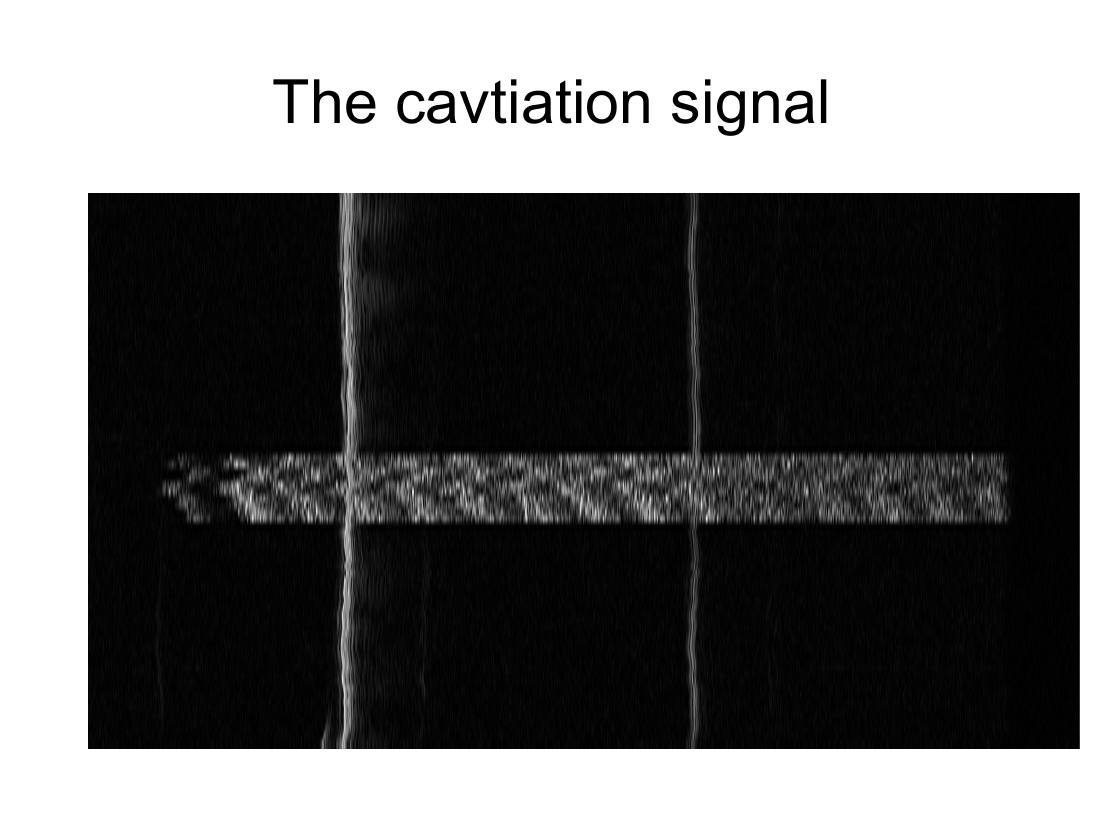
\includegraphics[width=0.8\textwidth]{emulsion_cavitation_signal.png}
%     \caption{Typical cavitation signal seen in bubbly water.
%     The two long vertical lines are the reflections of the sample
%     holder.
%     The imaging transducer is to the left,
%     the low-frequency transducer is to the right.}
%   \label{fig:cavitation}
%\end{figure}


%\begin{figure}[h]
%     \centering
%          
\includegraphics[width=0.8\textwidth]{pure90dbsmall41.png}
%     \caption{Typical cavitation signal seen in bubbly water.
%     The two long vertical lines are the reflections of the sample
%     holder.
%     The imaging transducer is to the left,
%     the low-frequency transducer is to the right.}
%   \label{fig:cavitation}
%\end{figure}



%%% Local Variables: 
%%% mode: latex
%%% TeX-master: "../../tshorrock_thesis"
%%% End: 

%  LocalWords:  Perfluorocarbon extravascularly
